\documentclass[11pt,]{article}
\usepackage{lmodern}
\usepackage{amssymb,amsmath}
\usepackage{ifxetex,ifluatex}
\usepackage{fixltx2e} % provides \textsubscript
\ifnum 0\ifxetex 1\fi\ifluatex 1\fi=0 % if pdftex
  \usepackage[T1]{fontenc}
  \usepackage[utf8]{inputenc}
\else % if luatex or xelatex
  \ifxetex
    \usepackage{mathspec}
  \else
    \usepackage{fontspec}
  \fi
  \defaultfontfeatures{Ligatures=TeX,Scale=MatchLowercase}
\fi
% use upquote if available, for straight quotes in verbatim environments
\IfFileExists{upquote.sty}{\usepackage{upquote}}{}
% use microtype if available
\IfFileExists{microtype.sty}{%
\usepackage{microtype}
\UseMicrotypeSet[protrusion]{basicmath} % disable protrusion for tt fonts
}{}
\usepackage[margin=1.0in]{geometry}
\usepackage{hyperref}
\hypersetup{unicode=true,
            pdftitle={Who are ASM Journals? A Gender-based Analysis},
            pdfborder={0 0 0},
            breaklinks=true}
\urlstyle{same}  % don't use monospace font for urls
\usepackage{graphicx,grffile}
\makeatletter
\def\maxwidth{\ifdim\Gin@nat@width>\linewidth\linewidth\else\Gin@nat@width\fi}
\def\maxheight{\ifdim\Gin@nat@height>\textheight\textheight\else\Gin@nat@height\fi}
\makeatother
% Scale images if necessary, so that they will not overflow the page
% margins by default, and it is still possible to overwrite the defaults
% using explicit options in \includegraphics[width, height, ...]{}
\setkeys{Gin}{width=\maxwidth,height=\maxheight,keepaspectratio}
\IfFileExists{parskip.sty}{%
\usepackage{parskip}
}{% else
\setlength{\parindent}{0pt}
\setlength{\parskip}{6pt plus 2pt minus 1pt}
}
\setlength{\emergencystretch}{3em}  % prevent overfull lines
\providecommand{\tightlist}{%
  \setlength{\itemsep}{0pt}\setlength{\parskip}{0pt}}
\setcounter{secnumdepth}{0}
% Redefines (sub)paragraphs to behave more like sections
\ifx\paragraph\undefined\else
\let\oldparagraph\paragraph
\renewcommand{\paragraph}[1]{\oldparagraph{#1}\mbox{}}
\fi
\ifx\subparagraph\undefined\else
\let\oldsubparagraph\subparagraph
\renewcommand{\subparagraph}[1]{\oldsubparagraph{#1}\mbox{}}
\fi

%%% Use protect on footnotes to avoid problems with footnotes in titles
\let\rmarkdownfootnote\footnote%
\def\footnote{\protect\rmarkdownfootnote}

%%% Change title format to be more compact
\usepackage{titling}

% Create subtitle command for use in maketitle
\newcommand{\subtitle}[1]{
  \posttitle{
    \begin{center}\large#1\end{center}
    }
}

\setlength{\droptitle}{-2em}

  \title{\textbf{Who are ASM Journals? A Gender-based Analysis}}
    \pretitle{\vspace{\droptitle}\centering\huge}
  \posttitle{\par}
    \author{}
    \preauthor{}\postauthor{}
    \date{}
    \predate{}\postdate{}
  
\usepackage{booktabs}
\usepackage{longtable}
\usepackage{array}
\usepackage{multirow}
\usepackage[table]{xcolor}
\usepackage{wrapfig}
\usepackage{float}
\usepackage{colortbl}
\usepackage{pdflscape}
\usepackage{tabu}
\usepackage{threeparttable}
\usepackage{threeparttablex}
\usepackage[normalem]{ulem}
\usepackage{makecell}
\usepackage{caption}

\usepackage{helvet} % Helvetica font
\renewcommand*\familydefault{\sfdefault} % Use the sans serif version of the font
\usepackage[T1]{fontenc}

\usepackage[none]{hyphenat}

\usepackage{setspace}
\doublespacing
\setlength{\parskip}{1em}

\usepackage{lineno}

\usepackage{pdfpages}
\floatplacement{figure}{H} % Keep the figure up top of the page
\usepackage{booktabs}
\usepackage{longtable}
\usepackage{array}
\usepackage{multirow}
\usepackage{wrapfig}
\usepackage{float}
\usepackage{colortbl}
\usepackage{pdflscape}
\usepackage{tabu}
\usepackage{threeparttable}
\usepackage{threeparttablex}
\usepackage[normalem]{ulem}
\usepackage{makecell}
\usepackage{xcolor}

\begin{document}
\maketitle

\vspace{35mm}

Running title: A gender-based analysis of ASM journals

\vspace{35mm}

Ada K. Hagan\({^1}\), Begüm D. Topçuoğlu\({^1}\), Hazel Barton\({^2}\),
Patrick D. Schloss\textsuperscript{1\(\dagger\)}

\vspace{40mm}

\(\dagger\) To whom correspondence should be addressed:
\href{mailto:pschloss@umich.edu}{\nolinkurl{pschloss@umich.edu}}

1. Department of Microbiology and Immunology, University of Michigan,
Ann Arbor, MI 48109

2. Department of Biology, University of Akron, Akron, OH

\newpage

\linenumbers

\subsection{Abstract}\label{abstract}

Evidence has accumulated over the decades that academic research has a
representation problem. While at least 50\% of biology Ph.D.~graduates
are women, the number of women in postdoctoral positions and
tenure-track positions are less than 40 and 30\%, respectively.
Recently, scientific societies and publishers have begun examining
internal submissions data to evaluate representation of, and bias
against, women in their peer review processes. However, representation
and attitudes differ by scientific field and no studies to-date seem to
have investigated academic publishing in the field of microbiology.
Using manuscripts submitted between January 2012 and August 2018 to 13
journals published by the American Society for Microbiology (ASM), we
describe the representation of women at ASM journals and the outcomes of
their manuscripts. We find that senior women authors at ASM journals are
underrepresented compared to global and society estimates of
microbiology researchers. Additionally, manuscripts submitted by
corresponding authors that were women, recieved more negative outcomes
(e.g., editorial rejections, reviewer recommendations, and decisions
after review), than those submitted by men. These negative outcomes were
somewhat mediated by whether or not the corresponding author was based
in the US or not and by the institution for US-based authors. However,
the trend for women corresponding authors to receive more negative
outcomes held, indicating a pattern of gender-influenced editorial
decisions.

\subsection{Importance}\label{importance}

Women are underrepresented as senior scientists at ASM journals. This is
due to a combination of both low submissions from senior women authors
and increased rejection rates for women compared to men.

\subsection{Introduction}\label{introduction}

Evidence has accumulated over the decades that academic research has a
representation problem. While at least 50\% of biology Ph.D.~graduates
are women, the number of women in postdoctoral positions and
tenure-track positions are less than 40 and 30\%, respectively
@article\{sheltzer\_elife\_2014\}. Studies examining other metrics such
as race and ethnicity find that less than 10\% of all science and
engineering doctorates were awarded to underrepresented minorities, and
less than 25\% of science and engineering doctorates in early career
academia identify as non-white (NSF ADVANCE, 2014). Predictably, the
disparities increase alongside academic rank
@article\{potvin\_diversity\_2018\}. There have been many proposed
reasons for these disparities, particularly with regards to women, that
include biases in training and hiring, the impact of children on career
trajectories, a lack of support for primary caregivers, a lack of
recognition, lower perceived comptency, and less productivity as
measured by research publications. \textbf{Add citations} These issues
do not act independent of each other, instead they are cumulative over
time for both individuals and the community. Accordingly, addressing
these issues necessitates multi-level approaches from all institutions
and members of the scientific community.

Scientific societies play an integral role in the formation and
maintenance of scientific communities. They host conferences that
provide a forum for knowledge exchange, networking, and opportunities
for increased visibility as a researcher. Scientific societies also
frequently publish the most reputable journals in their field,
facilitating the peer review process to vet new research submissions.
Recently, scientific societies and publishers have begun examining
internal submissions data to evaluate representation of, and bias
against, women in their peer review processes. The American Geological
Union found that while the acceptance rate of women-authored
publications was greater than publications authored by men, women
submitted fewer manuscripts than men and were used as reviewers only
20\% of the time (Lerback, 2017), a factor influenced by the gender of
the editor (Fox, 2016). Several other studies have concluded that there
is no significant bias against papers authored by women (C\&W, 2011;
Fox, 2016; Handly, 2015; Edwards, 2018). Two recent studies---one of the
peer review process at eLife, a broad scope biology journal, and the
other of outcomes at six ecology and evolution journals---found that
women-authored papers are less likely to have positive reviews and
outcomes (Murray, 2018; Fox and Paine, 2019).

However, representation and attitudes differ by scientific field and no
studies to-date seem to have investigated academic publishing in the
field of microbiology. The American Society for Microbiology (ASM) is
one of the largest life science societies, with an average membership of
41,000 since 1990. In its mission statement, the ASM notes that it is
``an inclusive organization, engaging with and responding to the needs
of its diverse constituencies'' and pledges to ``address all members'
needs through development and assessment of programs and services.'' One
of these services is the publication of microbiology research through a
suite of research and review journals. Between January 2012 and August
2018, ASM published 15 different journals: \emph{Antimicrobial Agents
and Chemotherapy} (AAC), \emph{Applied and Environmental Microbiology}
(AEM), \emph{Clinical and Vaccine Immunology} (CVI), \emph{Clinical
Microbiology Reviews} (CMR), \emph{Eukaryotic Cell} (EC),
\emph{Infection and Immunity} (IAI), \emph{Journal of Bacteriology}
(JB), \emph{Journal of Clinical Microbiology} (JCM), \emph{Journal of
Virology} (JV), \emph{mBio}, \emph{Microbiology and Molecular Biology
Reviews} (MMBR), \emph{Genome Announcements} (GA, now \emph{Microbiology
Resource Annoucements}), \emph{Molecular and Cellular Biology} (MCB),
\emph{mSphere} and \emph{mSystems}. We attempted to assign genders to
both peer review gatekeepers (e.g., editor-in-chief, editors, reviewers)
and authors on the original research manuscripts (eliminating CMR, GA,
and MMBR) evaluated during this time period. The goal of this research
study is to describe the representation of authors, reviewers, and
editors at ASM journals by gender and the associated peer review
outcomes of their manuscripts.

\subsection{Results}\label{results}

\textbf{Men dominate as gatekeepers and senior authors.} We first
evaluated the representation of men and women who were gatekeepers at
ASM during the study period. Each journal is led by an EIC who manages
journal scope and quality standards. In total, there were 17
editor-in-chiefs (EIC), 17.65\% of which were women. Two journals, EC
and CVI were retired during the period under study. In 2013, the
leadership of CVI transferred from a man EIC, to a woman. JVI has had
the same woman as EIC since 2012. The EICs manage a board of editors
with field expertise to handle the peer review process. The total number
of editors over the duration of our study (senior editors and editors
pooled) was 1016 and 28.74\% were women.

Over 40\% of both men and women editors were from US-based R1
institutions, with non-US and medical schools and institutions supplying
the next largest proportions of editors (Fig. 1A). Since the start of
our study, there has been a slow trend toward equivalent gender
representation among editors (Fig. 1B). The trends for each journal
studied vary considerably, though most have slow trends toward parity
(Fig. S1). CVI and \emph{mSphere} were the only ASM journals to have
accomplished equivalent representation of both genders, with CVI having
a greater proportion of women editors than men before it was retired. EC
is the only journal with an increasing parity gap.

Our data set contained \# of manuscripts each of which contained a list
of potential reviewers. A total of 30704 reviewers, 24.61\% of which
were women, agreed to act as reviewers when contacted. The greatest
proportion of reviewers (over 50\% of both men and women) come from
non-US institutions, while R1 institutions supply the next largest
cohort of reviewers (Fig. 1C). Over the time period studied, the
proportions of each gender have held steady among reviewers at ASM
journals (Fig. 1D) and is representative of both reviewer proportions at
each journal, and the potential reviewers at all journals combined (Fig.
S2).

\textbf{Editorial workloads were not proportionate} Across all journals,
men handle a slightly greater proportion of manuscripts (blue) and women
a slightly smaller proportion (orange), relative to their respective
editorial representations (Fig. 1A). This trend continues across most
journals with varying degrees of difference between workload and
representation (Fig. S1). There were exceptions. At \emph{mSphere},
workload and proportions were identical. However, CVI, \emph{mBio}, and
JVI, each have points at which the workload for women editors is much
higher than their representation, with corresponding decreases in the
workload of men. In the years preceding its retirement, the
representation of women at CVI increased, which acted to decrease the
gap with their workload. However, representations and relative workloads
for men and women editors at JVI have held steady over time, while the
proportionate workload for women at \emph{mBio} has increased.

Between 2012 and 2018, the median number of manuscripts reviewed by
individuals in each gender group is equivalent at 2. Half of men, women,
and unknown genders reviewed between one and 5, 4, or 3 manuscripts
each, respectively (Fig. 2B). 43.35, 38.97, and 47.45\% of men, women,
and unknown reviewers have reviewed only one manuscript (Fig. 2C).
Reviewers of all genders, accepted fewer requests to review from women
editors (average of 47.9066667\%) than men (average of 53.4\%) and were
less likely to respond to women than men (average of 25.04 and 19.91\%,
respectively) (Fig. 2C). Editors of both genders contacted reviewers
from all three gender groups at equivalent proportions, though women
editors contact 76.29\% of potential reviewers, compared to men who
contact 73.92\% (Fig. 2D).

\textbf{Women were underrepresented as authors} Globally, microbiology
researchers are 60\% men and 40\% women (Elsevier report). At ASM in
September 2018, 38.37\% of members who reported their gender were women.
We wanted to determine if these proportions were similar for authors at
ASM journals and to understand the distribution of each gender among
submitted and published manuscripts. We began by describing author
institutions by gender. Over 60\% of authors were from non-US
institutions, followed by 20\% from R1 institutions (Fig. 3A). The
proportions of men and women authors at ASM have decreased over time at
equivalent rates, with a ratio of men to women authors of 4:3 since 2012
(or, 57\% men) (Fig. 3B). This decrease corresponds with an increase in
the proportion of unknown gendered authors.

The proportion of papers submitted with men and women first authors have
remained constant with an average of 29.64 and 31.08 percent,
respectively (Fig. 3C). Their respective proportions of average
published manuscripts were nearly identical at 33.16\% for men and
33.85\% for women. The proportion of submitted papers with men
corresponding authors (defined in the methods) has remained steady at an
average of 42.45\% and the proportion with women corresponding authors
at 23.56\%. However, their respective proportions of published
manuscripts, 49.85\% for men and 24.35\% for women, were dissimilar
(Fig. 3D). The difference between published and submitted proportions of
manuscripts where men were corresponding authors is 7.4, and 0.79 for
women corresponding authors. This trend is similar for middle and last
authors (Fig. S3).

Of 39168 manuscripts submitted by men corresponding authors (single
author papers excluded), 23.52\% had zero women authors. 7403 (36.45\%)
of papers submitted by women corresponding authors have at least 51\% of
the authors as women, exceeding those submitted by men corresponding
authors, 3305 (8.44\%). We also found that the proportion of women
authors decreases as the number of authors increases (Fig. S4). To
verify that the trend is non-random, we ran a logistic regression model
predicting the gender of the corresponding author. Variables of the
model included whether or not the corresponding author's institution was
in the U.S. or not, the total number of authors, the proportion of
authors that were women, whether or not the article was published, the
gender of senior editors and editors, the number of revisions, and
whether or not the manuscript was editorially rejected. Single author
manuscripts and those with either all men or all women authors were
excluded. The value of the area under the curve (AUC), for this model
was 0.7. The AUC value ranges between one and zero, where the
reliability of the prediction model increases with the AUC. The primary
predictive driver of this model was the proportion of women authors on a
paper, with a median weight of -3.64. All other variables had weights
less than 1, indicating little to no influence on the model.

To better visualize the 7.52 decrease in the proportion of women who
were first authors to those who were corresponding authors (Fig. 3CD),
we asked the proportions at which women have been retained through the
peer review system at ASM journals. During the period of time under
study, there were 76215 women who participated as junior authors (first,
middle) at ASM journals. Of those junior authors, 8.25\% also
participated as senior authors (last, corresponding), and 8.91\% were
listed as potential reviewers. 5.39\% of the women junior authors
participated as reviewers and, 0.25\% held a role as editor. For men,
there were a total of 84482 junior authors, where 13.59 were also senior
authors, 16.72 considered as reviewers, and 11.11 actually reviewed.
0.66 of men junior authors were also editors at ASM journals.

\textbf{Papers submitted by women have more negative outcomes than those
submitted by men.} To better understand the differences between
published and submitted proportions for men and women authors (Fig. 3CD,
Fig. S3), we next compared the rejection rates of men and women at each
author stage (e.g., first, middle, corresponding, and last). Middle
authors were rejected at similar rates for men and women, a 0.11
percentage point difference across all journals combined. However,
manuscripts with senior women authors were rejected more frequently than
those authored by men with -2.26 and -1.2 percentage point differences
for corresponding and last authors, respectively (Fig. 4A). Breaking it
down by individual journals, there were several instances where the
overall trend is repeated or even amplified (e.g., AAC, IAI, JB,
\emph{mBio}, MCB). The greatest effect was observed when comparing the
gender of corresponding authors, so we used this sub-population to
further examine the difference in acceptance/rejection rates.

We next compared the rejection rates for men and women corresponding
authors after two bottlenecks, initial review by the editor and the
first peer review. Papers authored by women were editorially rejected as
much as 12 percentage points more often than those authored by men (Fig.
4B). The percentage point difference at all ASM journals combined is
-3.87 (vertical line), and two journals, MCB and \emph{mBio}, have more
extreme percentage point differences. Papers authored by men and women
were equally likely to be accepted after the first round of review (Fig.
4C, right panel). However, women-authored papers were rejected more
often (left panel) while men-authored papers were more often given
revision decisions (center panel). Three journals, JB, AAC, and MCB,
have percentage point differences more extreme than for all ASM journals
combined in both rejection (-5.5) and revision (5.46) decisions
(vertical lines).

In addition to manuscript decisions, other disparate outcomes may occur
during the peer review process. To determine whether women-authored
papers spent more time between being submitted and ready for
publication, we compared the number of revisions, days spent in the ASM
peer review system, and the number of days from submission to being
ready for publication to those authored by men. Papers authored by women
take slightly longer (from submission to ready for publication) than men
at some journals ( \emph{mSphere}, \emph{mBio}, \emph{mSystems}, CVI,
JB, JCM, AEM) despite spending similar amounts of time in the ASM
journal peer review system, and having equivalent median number of
revisions prior to acceptance (Fig. S5).

To understand how gatekeeper (editor/reviewer) genders influence
decisions (e.g., Fig. 4C), we grouped editor decisions and reviewer
suggestions according to the gatekeeper gender. Both men and women
editors rejected proportionally more women-authored papers, with men
editors making revise decisions on papers authored by men more often
than those authored by women (Fig. 5A). Reviewers were more likely to
suggest rejections for women as compared to men, though no difference in
revise suggestions were observed (Fig. 5B). Both men and women reviewers
recommended rejection more often for women-authored manuscripts though
only men recommended acceptance more often for men-authored manuscripts
(Fig. 5C). Women reviewers suggested revision on women-authored papers
more often than men-authored manuscripts.

To evaluate whether or not manuscript decisions were random when gender
is taken into account, we used a logistic regression model to predict
whether or not a manuscript was reviewed (i.e., editorially rejected or
not). When accounting for the genders of the senior editor, editor, and
corresponding author, as well the proportion of authors that were women,
the median AUC of this model was 0.62. Because the AUC value was above
0.6, the editorial rejection decisions were not completely random,
though the model reliability is low. This suggests that other factors
influence gender-based decisions.

\textbf{Country and institute of origin contribute to overperformance by
men.} The issue of non-random, gender-based manuscript decisions could
be attributed to gender bias by journal gatekeepers, however, there are
other types of bias that may contribute to, or obscure, overt gender
bias. For instance, a recent evaluation of peer-review outcomes at
\emph{eLife} found evidence of geographic homophiliy, that is, reviewers
exhibited preference for research submitted by authors from their own
country or region (Murray, 2019). Other studies have documented prestige
bias, where men are over-represented in more prestigious (i.e., more
respected and competent) programs (Weeden, 2017). It is therefore
possible, that what seems to be gender bias could be geographic or
prestige bias interacting with the increased proportion of women
submitting from outside the US or at lower prestige institutions (e.g.,
low research institutions) (Fig. 3A).

To try to separate how these factors affect manuscript decisions among
corresponding authors, we next looked at the outcome of papers submitted
only by corresponding authors at US institutions. When only considering
US-based authors, the difference in percentage points for editorial
rejections changes from -3.87 to -1.51, though trends across journals
were consistent (Fig. 6A). Similarly, trends in the difference in
percentage points of decisions after review for US-based authors mirror
those seen for all corresponding authors at the journal level in Figure
4B. Though there were changes in the values for all journals combined.
The over-performance of women in rejection decisions decreases from -5.5
to -3.39, and the over-performance of men in revise only decisions from
5.46 to 3.43 (Fig. 6B). The rate of accept decisions changed from -3.87
to -0.05 after restricting the analysis to US-based authors. These
results suggest that the country of origin (e.g, US versus not) accounts
for some gender bias, particularly for editorial rejections, but not all
of it.

To address prestige bias, we next split the US-based corresponding
authors according to their institution and re-evaluated the difference
in percentage points for men and women. Editorial rejections occurred
most often for women from medical schools or institutes, followed by
those from R2 institutions (Fig. 6C). Manuscripts submitted by men from
medical schools or institutes were accepted proportionally more often
than those submitted by women. The difference in percentage points for
corresponding authors from medical schools or institutes seems to be
spread across most ASM journals, while the editorial rejection of papers
from R2 institutions seems to be driven primarily by JCM (Fig. S6AB).
The occurrence of rejections after review occurred more often for
manuscripts submitted by women than those submitted by men, regardless
of editor gender (Fig. 6D). There were a couple of exceptions where
women authors from low research and industry research institutions
received more positive decisions by men editors.

Corresponding authors who were men from non-US institutions consistently
over-perform compared to women from non-US institutions. About 15
percentage points more manuscripts submitted by men from non-US
institutions were accepted after review, than those submitted by women
(Fig. 6C). Editors that were men rejected 20 percentage points more
manuscript submitted by women than those submitted by men, whereas the
difference for women editors is much smaller at -5 (Fig. 6D). These
trends amplify those seen from difference in percentage points of review
recommendations (Fig. S6CD).

To understand if these factors affect manuscript decisions in a
non-random manner, we used logistic regression model that took into
account both origin (US vs non), institution (US institution type),
number of authors, proportion of authors that were women, and the
genders of both gatekeepers and authors. This model predicted whether or
not a manuscript was editorially rejected and had a median AUC of 0.68
indicating non-random interaction between these factors. Those factors
with the greatest positive impacts (i.e., increased likelihood of
editorial rejection) were US Inst Type Other, Sen Editor Men, Other US
Inst Men, Med School \& Institutes Women. The factors with the greatest
negative impacts (i.e., increased liklihood of going to review) were R1
Univ, US, Sen Editor Women, Num Authors. These results confirm that the
country of origin and prestige bias impact decisions in a non-random
manner, but gender-based factors were still at play.

\subsection{Discussion}\label{discussion}

In this paper we described the representation of men and women at ASM
journals between January 2012 and August 2018, and compared editorial
outcomes according to the author gender. We found that women were
consistently represented at 30\% or less in all levels of the peer
review process, excluding junior authors where women were X percent.
Women and men editors had proportionate workloads accross all ASM
journals combined, but those workloads were disproportionate at the
journal level and the overburdened group varied according to the
journal. Additionally, manuscripts submitted by corresponding authors
that were women, recieved more negative outcomes (e.g., editorial
rejections, reviewer recommendations, and decisions after review), than
those submitted by men. These negative outcomes were somewhat mediated
by whether or not the corresponding author was based in the US or not
and by the institution for US-based authors. However, the trend for
women corresponding authors to receive more negative outcomes held,
indicating a pattern of gender-influenced editorial decisions.

While the proportion of women as first authors is equivalent to data
obtained globally from self-reported at ASM, it was higher than the
proportion of senior women authors at ASM journals. Additionally, half
as many women than men who were junior authors at ASM journals were also
senior authors and the representation of women decreased as the status
(e.g., reviewer, editor) increased. These observations are consistent
with for representation of senior women in academic biological sciences
and the observation that women are more likely to leave academia during
the transition from postdoc to investigator (Martinez, 2007). These data
indicate that microbiology (as represented by ASM journals) is not
exempt from the so-called ``leaky pipeline''.

How to define representation and determine what the leadership should
look like are recurring questions in STEM. We argue that if all things
were considered equal than representation for men and women
corresponding authors, reviewers, and editors would be at about 50\%
each. However, that is not (yet) the case, so we argue that the goal
should depend on the workload and visibility of the position(s). Since
high visibility positions (e.g., editor, EIC) are filled by a smaller
number of individuals that are responsible for recruiting more
individuals into leadership, filling these positions should be done
aspirationally (i.e., 50\% should be women if the goal were an
aspirational leadership. ). This allows expansion of the potential
reviewer network and thus recruitment into those positions. Conversely,
lower visibility positions (e.g., reviewers) require a greater number of
individuals and should thus be representational of the field to avoid
overburdening the minority population (i.e., since 23.5\% of
corresponding authors to ASM journals are women, then 23-24\% of
reviewers should be women). Balancing the workload is particularly
important given the literature indicating that women faculty have higher
institutional service loads than their counterparts who are men.

In contrast to institutional service, the editing workload at ASM
jounals seems to be predominantly borne by men, according to the
proportion of representation. Possible explainations for the difference
in gatekeeper representation and editor workloads could be that women
are more likely to conduct research on the fringes of research fields.
Their separation from the historical center of a field decreases their
percieved competency, which could result in research typecasting and
lower manuscript handling responsibilities. Other posibilities are that
the increased service load decreases their ability to handle larger
editorial loads or that since status as an editor is ``prestigous'', the
workload is prefferentially diverted to editors that are men. Any of
these situations can be compounded by the increased proportion of
potential reviewers that either do not accept, or do not respond to,
requests to review from women editors. This increases the proportion of
reviewers that women editors must contact, adding additional time and
work to their editorial burdens. Three journals, \emph{mBio}, CVI, and
JVI are exceptions with regards to editorial workloads. At these
journals, the editorial workloads of women exceeds their representation.
A possible explaination for CVI and JVI is that both of these journals
have been led by women EICs, who perhaps have increased confidence in
their women editors. Alternately, the tendency for reviewers to reject
requests to review from editors that are women extends to editors that
are men rejecting requests to handle manuscripts from EiCs that are
women. Our data differ from those of Fox, 2016(?) who found that the
gender of the contacted reviewer depended on the gender of the editor,
but supports findings X are less likely to respond to requests from
editors that are women.

Our data also supports previous studies finding that women are more
likely to collaborate with other women and that women are less likely to
be on highly collaborative papers. In our linear regression models, the
number of authors on a manuscript was the largest contributor to
avoiding editorial rejections, suggesting that highly collaborative
research is preferred by editors. It is, therefore, disturbing that when
the number of authors exceed 30 on a manuscript, the proportion of women
is always below 51\%, despite equivalent numbers of trainees in the
biological sciences (Fig. S4). Additionally, while women corresponding
authors submit fewer papers, more of them, both numerically and
proportionally, have more than 50\% women authors, compared to those
submitted by men corresponding authors. Previous research suggests that
women who collaborate with other women recieve less credit for these
publications than when they collaborate with men (Wiedman, 2019), and
that women are more likely to yield corresponding authorship to
collegues that are men (Fox). The gender-based segregation of
collaborations at ASM journals has consequences in pay and promotion and
could be a factor in the decreased retention of senior women at ASM
journals.

The under representation of women as corresponding authors in
publication at ASM journals has negative consequences for their careers
and microbiology since it is their role as a senior author that impacts
their status in the field. Buckley et al, suggest that being selected as
a reviewer increases visibility of a researcher, which has a direct \&
significant impact on salary. Therefore, the under representation of
women as senior authors and reviewers hampers their career progression
and even their desire to progress since status in the peer review
process also signals adoption of the researcher into the scientific
community (Buckley et al, 2014). Retention of women in science is
important to the progress of microbiology as a field since less
diversity in researchers limits the diversity of perspectives,
approaches, and thus stunts the search for knowledge. In addition to
boosting productivity and knowledge, more diverse and equitable
organizations are more inclusive and supportive for all members (Potvin,
2018).

The support of academic research journals for women has been the topic
of many papers, which note the lack of women authors relative to men.
However, submissions data is required to determine if the lack of
representatiion is due to low submissions or bias during peer review. We
have shown that there is a disparity in submissions from senior women in
microbiology compared to men, but this does not fully account for the
difference in publications by men and women corresponding authors at ASM
journals. There is also a consistent trend favoring positive outcomes
for manuscripts submitted by corresponding authors that are men over
women. Manuscripts submitted by corresponding authors who are women are
editorially rejected at greater rates than those submitted by men, and
gatekeepers of both genders favor revisions for manuscripts authored by
men than by women. Neither geographic (e.g., US or not) nor prestige
bias can fully account for the gender-based bias observed.

We do not have sufficient data to determine the specific nature of the
implicit biases observed, but there are several possibilites. Curiously,
while the median of manuscript versions before publication is identical
for both men and women, manuscripts authored by women have increased
rejection rates and time between submission and publication. This
suggests that manuscripts submitted by women are given more revisions
(i.e., work) from reviewers and/or their competency to complete
revisions within the prescribed 30 days is doubted, compared to men.
This observation fits with previous studies documenting that a greater
burden of proof is required for women to achieve similar competency as
men (Blair-Loy, 2017). Even if a gatekeeper doesn't personally know the
corresponding author, women and men have adopted different writing
styles that can act as cues to the author's gender. In particular, the
increased requirements of competency for women leads to manuscripts with
increased explanations and detail than those authored by men (Kolev,
2019; Erin). Finally, significant time, funds, and staff are required to
be competitive in highly active fields (e.g., \emph{Clostridium
difficile}, HIV), but women are often at a disadvantage for these
resources due to the cumulative affects of bias (cites). As a result,
corresponding authors that are women may be spending their resources at
the lesser competitive fringes of research fields (\textbf{citation}).
This has the disadvange of further decreasing percieved competency to
those at the established center of the field in turn increasing the
difficulty to obtain funding and publish in more traditional journals.

Few papers have found disparities between rejection rates of men and
women and to our knowledge, this is the first paper to collectively
examine this issue with either submissions data from this many journals
or on the field of microbiology. Critics might argue that the effect
size is too small to really matter. However, the consistency of the
trends to benefit men corresponding authors over women, across all
journals included in this study and literature to-date confirms that
this descriptive study is highly relevant for the ASM as a society. Our
findings offer opportunities to address gendered representation in
microbiology and systemic barriers to peer review at our journals.

\subsection{Data and Methods}\label{data-and-methods}

\textbf{Data} All manuscripts handled by ASM journals (e.g.,
\emph{mBio}, \emph{Journal of Virology}) that received an editorial
decision between January 1st, 2012 and August 31st, 2018 were supplied
as XML files by ASM's publishing platform, eJP. Data were extracted from
the XML documents provided using R statistical software (version 3.4.4)
and the XML package (R citation). Data manipulation was handled using
the tidyverse, lubridate, and xml2 packages for R. Variables of interest
included: the manuscript number assigned to each submission, manuscript
type (e.g., full length research, erratum, editorial), category (e.g.,
microbial ecology), related (i.e., previously submitted) manuscripts,
number of versions submitted, dates (e.g., submission, decision), author
data (e.g., first, last, and corresponding authorship, total number of
authors), reviewer data (e.g., reviewer score, recommendation, editor
decision), and personal data (names, institutions, country) of the
editors, authors, and reviewers. For this analysis, only original,
research-based manuscripts were included, e.g., long- and short-form
research articles, New-Data Letters, Observations, Opinion/Hypothesis
articles, and Fast-Track Communications.

Data were visualized using the ggplot, scales, RColorBrewer, and
ggalluvial packages for R.

\textbf{Defining manuscript outcomes} Many papers are immediately
rejected by editors/EICs instead of being sent to peer review, often due
to issues of scope or perceived quality. These were defined as editorial
rejections and identified as manuscripts rejected without record of
review. Alternately, editors could send papers out for review by two or
three experts in the field. The reviewers make suggestions to the editor
who decides whether the manuscript in question should be accepted,
rejected, or sent back for revision. At ASM journals, manuscripts with
suggested revisions that are expected to take more than 30 days are
rejected, but generally encouraged to resubmit. If resubmitted, the
authors are asked to note the previous (related) manuscript and the
re-submission is assigned a new manuscript number. Multiple related
manuscripts were tracked together by generating a unique grouped
manuscript number based on the recorded related manuscript numbers. This
grouped manuscript number served multiple purposes including: tracking a
single manuscript through multiple rejections or transfers between ASM
journals and to avoid duplicate counts of the same authors for the same
manuscript.

\textbf{Institution classification} To identify the communities
represented, we used Carnegie classifications to group US-based
institutions into R1, R2, low (not R1 or R2), and medical research.
Research institutes, industry, and federal research groups were
identified using the internet. Medical schools and institutions (e.g.,
Mayo clinic) were grouped together. Industry and federal research were
grouped separately. The ``Other'' category represents uncategorized US
institutions. Non-US institutions are a category on their own.

\textbf{Manuscript outcome analysis and presentation} In the field of
microbiology, order of authorship on manuscripts signal the type and
magnitude of contributions to the finished product with first and last
authorship being the most prestigious. First authors are assumed to be
trainees (e.g., students or post-docs) responsible for the bulk of the
project, while last authors are lead investigators, supplying conceptual
guidance and resources to complete the project. Middle authors are
generally responsible for technical analyses and methods. Any author can
also be a corresponding author, which can be defined as either the
individual to whom questions are directed by readers or the individual
responsible for communicating with publishing staff during peer review.
We use the latter definition for our analysis.

To better visualize and understand the differences in outcomes according
to author gender, we calculated the difference in percentage points
between the proportion of that outcome for men and women. To correct for
the disparity in the participation of women relative to men at ASM
journals, all percentage point comparisons are made relative to the
gender and population in question. For instance, the percentage point
difference in acceptance rates is the acceptance rate for men minus the
acceptance rate for women. A positive value indicates that men receive
the outcome more often than women, whereas a negative value indicates
that women outperform men in the given metric.

\textbf{Logistic regression models} For the L2-regularized logistic
regression models, we established modeling pipelines for a binary
prediction task. First, we randomly split the data into training and
test sets so that the training set consisted of 80\% of the full data
set while the test set was composed of the remaining 20\% of the data.
To maintain the distribution of the 2 model outcomes that was found with
the full data set, we performed stratified splits. The training data was
used to build the models and the test set was used for evaluating
predictive performance. To build the models, we performed an internal
five-fold cross-validation where we tuned the cost hyper-parameter,
which determines the regularization strength where smaller values
specify stronger regularization. This internal cross-validation was
repeated 100 times. Then, we trained the full training data set with the
selected hyper-parameter values and applied the model to the held-out
data to evaluate the testing predictive performance of each model. The
data-split, hyper-parameter selection, training and testing steps were
repeated 100 times to get a reliable and robust reading of model
performance. Models were trained using the machine learning wrapper
caret package (v.6.0.81) in R (v.3.5.0).

\textbf{Gender prediction and assignment} The gender assignment API
genderize.io was used to predict an individual's gender based on their
given names, and country where possible. The genderize.io platform uses
data gathered from social media to predict gender based on given names
with the option to include an associated language or country to enhance
the odds of successful prediction. Since all manuscripts are submitted
in English, precluding language association for names with special
characters, names were standardized to ASCII coding (e.g., ``José'' to
``Jose''). We next matched each individuals country against the list of
X country names accepted by genderize.io. Using the
\texttt{GenderGuesser} package for R, all unique given names associated
with an accepted country were submitted to the genderize.io API and any
names returned without a predictive assignment of either male or female
were resubmitted without an associated country. All predictive
assignments of either male or female are returned with a probability
match of 0.50 or greater. The predicted genders of all given names (with
and without an associated country) whose probabilities were greater or
equal to our arbitrary success cut off of 0.65 were used to assign
predicted gender to the individuals in our data set. Predicted genders
were assigned to individuals in the following order: first names and
country, first names, middle names and country, middle names (Fig. S7).
The presenting gender (man/woman) of editors and senior editors in our
data set was hand validated using Google where possible.

We recognize that biological sex (male/female) is not always equivalent
to the gender that an individual presents as (man/woman), which is also
distinct from the gender(s) that an individual may self-identify as. For
the purposes of this manuscript, we choose to focus on the presenting
gender (man/woman/unknown) based on their first names and/or appearance
(for editors). In the interest of transparency, we include those
individuals whose names don't allow a high degree of confidence for
gender assignment in the ``unknown'' category of our analysis.

\textbf{Validation of gender prediction} We first validated the
algorithm using a set of 3265 names whose gender had been hand-coded
based on appearance (Broderick \& Casadevall cite). The names were
supplied to the genderize algorithm both with and without the
accompanying country data. The data returned include the name, predicted
gender (male, female, na), the probability of correct gender assignment
(ranging from 0.5 to 1.0), and the number of instances the name and
gender were associated together (1 or greater). The genderize algorithm
returned gender predictions for 2899 when first names were given and
2167 when country data was also supplied (732 names were associated with
countries unsupported by genderize).

Sensitivity and specificity, are measurements of the algorithm's
tendency to return correct answers instead of false positives (e.g., a
man incorrectly gendered as a woman) or false negatives (e.g., a woman
incorrectly gendered as a man). The closer these values are to 1, the
smaller the chance that the algorithm will return the correlating false
response. Accuracy is a composite measure of the algorithm's ability to
differentiate the genders correctly. These measurements were calculated
from the data sets (with and without country data supplied) at three
different probability threshold cutoffs: the default genderize (0.5), a
probability threshold of 0.85 (0.85), and a modified probability of
0.85, which factors in the number of instances returned
(pmod0.85)(citations).

At the 0.5 threshold, the data set returned a sensitivity of 0.8943 and
specificity of 0.9339 for an accuracy of 0.911, compared to a marginally
higher accuracy of 0.9146 for the data set where country data were
included (Table S1). Generally speaking, the accuracy increases as the
threshold increases along with slight trade offs between sensitivity and
specificity. For the purposes of our analysis, we opted to use the
pmod0.85 threshold moving forward (Table S1, in bold).

To understand the extent of geographic bias in our gender assignment
against regions and languages with gender-less naming conventions, or
that lack social media for incorporation into the genderize algorithm,
we compared the number of names predicted without associated country
data to when country data was also supplied. In our test data set, the
top five countries associated with names were United States, Germany,
United Kingdom, France, China and the countries with the highest
proportion of un-predicted genders when country data were supplied are
Cambodia, Iceland, Indonesia, Ireland, Mexico, where the maximum number
of names supplied ranged from 1 to 15. To determine the impact of each
country towards the overall percentage of names whose genders were not
predicted (27.14\%), we found the difference between the percent of
names un-predicted for each country and the overall percentage,
multiplied by the proportion of observations from that country to the
total observations and finally divided by the overall percentage of
un-predicted names (Fig. S8). The top five countries with the greatest
impact on un-predicted names, and thus the countries receiving the most
negative bias from genderize were Canada, China, Ireland, Belgium,
Sweden (Fig. S9). These data suggest that there is likely some bias
against countries with gender-neutral naming conventions (China), and
indicates the stringency with which the algorithm applies gender to
names that are accompanied by country data. For instance, strongly
gendered names such as Peter and Pedro were not assigned gender when
associated with Canada.

We next applied the genderize algorithm at the pmod0.85 threshold to our
journals data set and tested its validity on a small portion. All first
names collected from our data set were submitted to genderize both with
and without country data. Only those predictions whose pmod were
equivalent or greater than 0.85 were carried to the next step. The
predicted genders were assigned to individuals in the following order:
first names and country, first names, middle names and country, middle
names. Given the relatively small number of editors and senior editors
in our data set, the presenting gender (man/woman) of editors and senior
editors in our data set was hand-validated using Google where possible.
Of the 1072 editor names, 938 were predicted by genderize for an
accuracy of 0.9989339, thus increasing our confidence in the gender
predictions where made.

In our full data set, the five countries with the most individuals were
United States, China, Japan, France, Germany and the countries with the
highest proportion of un-predicted genders were Burundi, Chad, Kingman
Reef, Korea (North), Democratic People's Republic of, Maldives, where
the maximum number of names supplied ranged from 1 to 4. Proportionally,
fewer names in our full data set were assigned gender than in our
validation data set (40.01\% un-predicted versus 27.14\% un-predicted,
respectively). Since adjusting the workflow to predict the gender of
names both with and without country data, the countries receiving the
most negative bias from genderize were China, Japan, Korea, Republic of,
India, Taiwan, Province of China (Fig. S10). These data indicate what we
previously predicted, that the genderize algorithm has bias against
countries with gender-neutral naming conventions.

\textbf{Code and data availability} Anonymized data and code for all
analysis steps, logistic regression pipeline, and an Rmarkdown version
of this manuscript, is available at
\url{https://github.com/SchlossLab/Hagan_Gender_mBio_2019/}

\textbf{Acknowledgements} We would like to thank Nicole Broderick and
Arturo Casadevall for providing their data set for genderize validation
and acknowledge Arianna Miles-Jay and Joshua MA Stough for their
comments.

A.K.H. was responsible for project and experiment design, data analysis,
and drafting the manuscript. B.T. completed the logistical regression
models. P.D.S. provided funding, resources and conceptual advice. All
authors contributed to the final manuscript. P.D.S. is Chair of ASM
Journals and A.K.H. was ASM staff prior to publication of the analysis.
B.T. reports no conflict of interest.

Funding for this work was provided by the American Society for
Microbiology. The sponsors had no role in study design or
interpretation.

\newpage

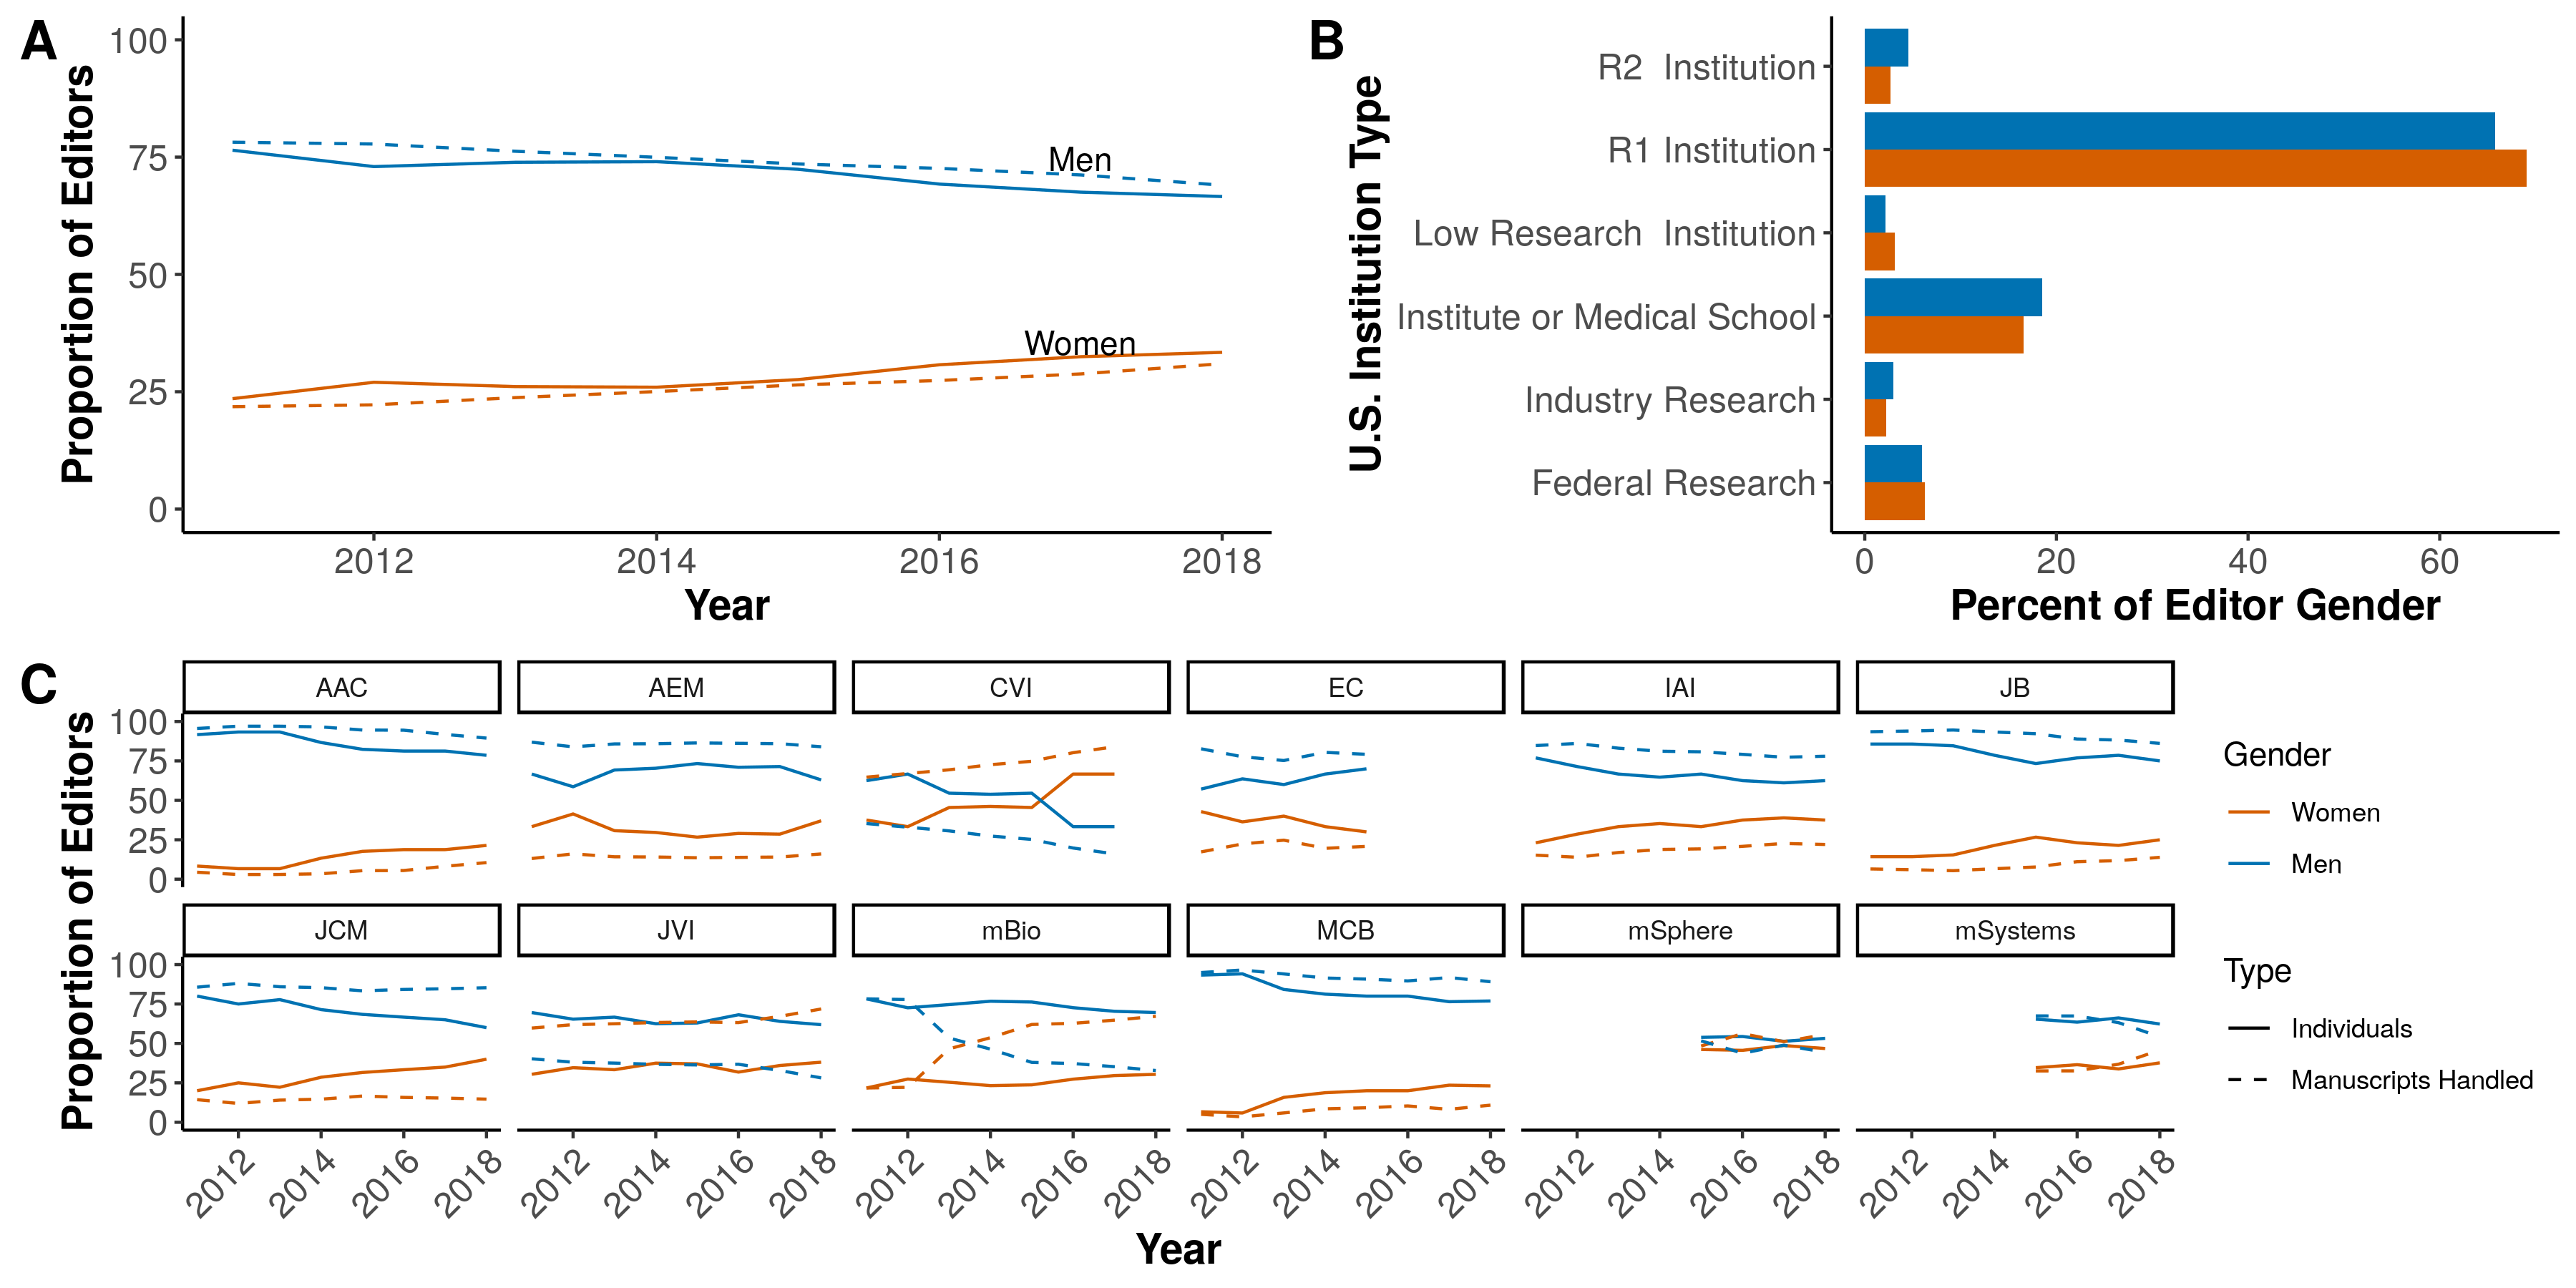
\includegraphics{Figure_1.png} \textbf{Figure 1. Gendered representation
among gatekeepers.} Proportion of editors from (A) institution types and
(B) over time from 2012 to 2018. Editors and senior editors are pooled
together. Proportion of reviewers from (C) institution types and (D)
over time from 2012 to 2018. (A,C) Institutions within each gender add
to 100\%.(B,D) Each individual was counted once per calendar year,
proportions of each gender add to 100\% per year.

\newpage

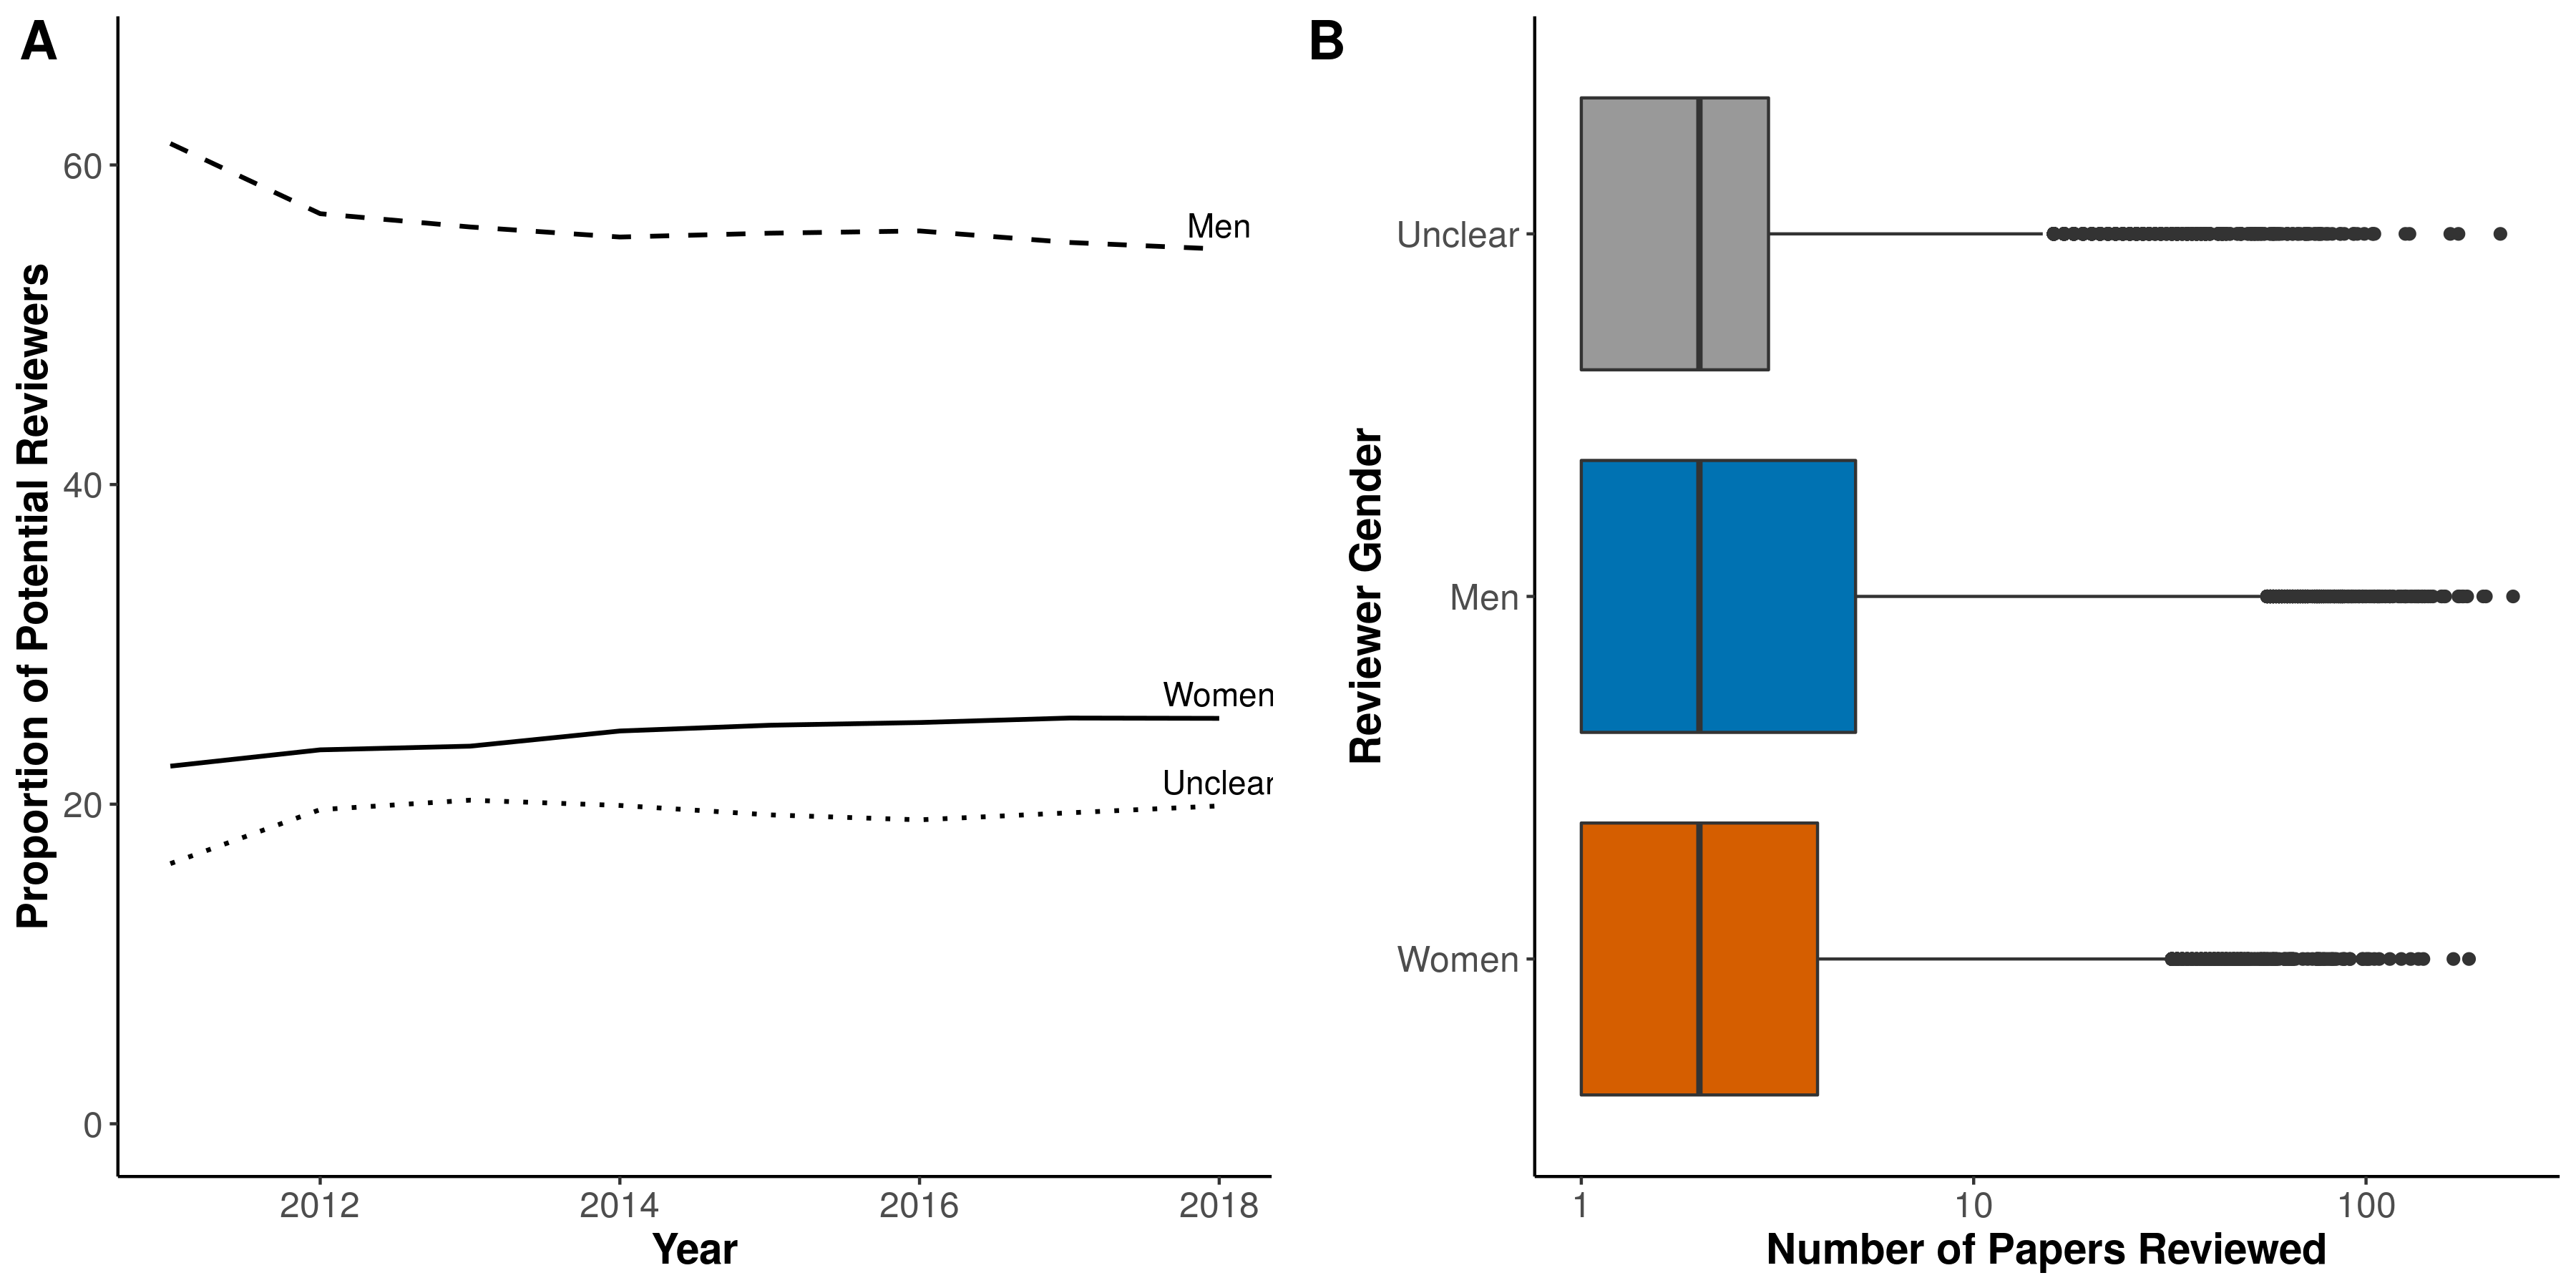
\includegraphics{Figure_2.png} \textbf{Figure 2. Gatekeeper workload and
response to requests to review.} (A) Proportion of manuscript workloads
by men and women editors, editorial rejections excluded. (B) Box plot
comparison of total manuscripts reviewed by each individual according to
gender. (C) The percent of reviewers by gender that either accepted the
opportunity to review or did not respond to a request to review, split
according to the editor's gender. (D) Percent of each potential reviewer
gender contacted to review, according to the editor's gender.

\newpage

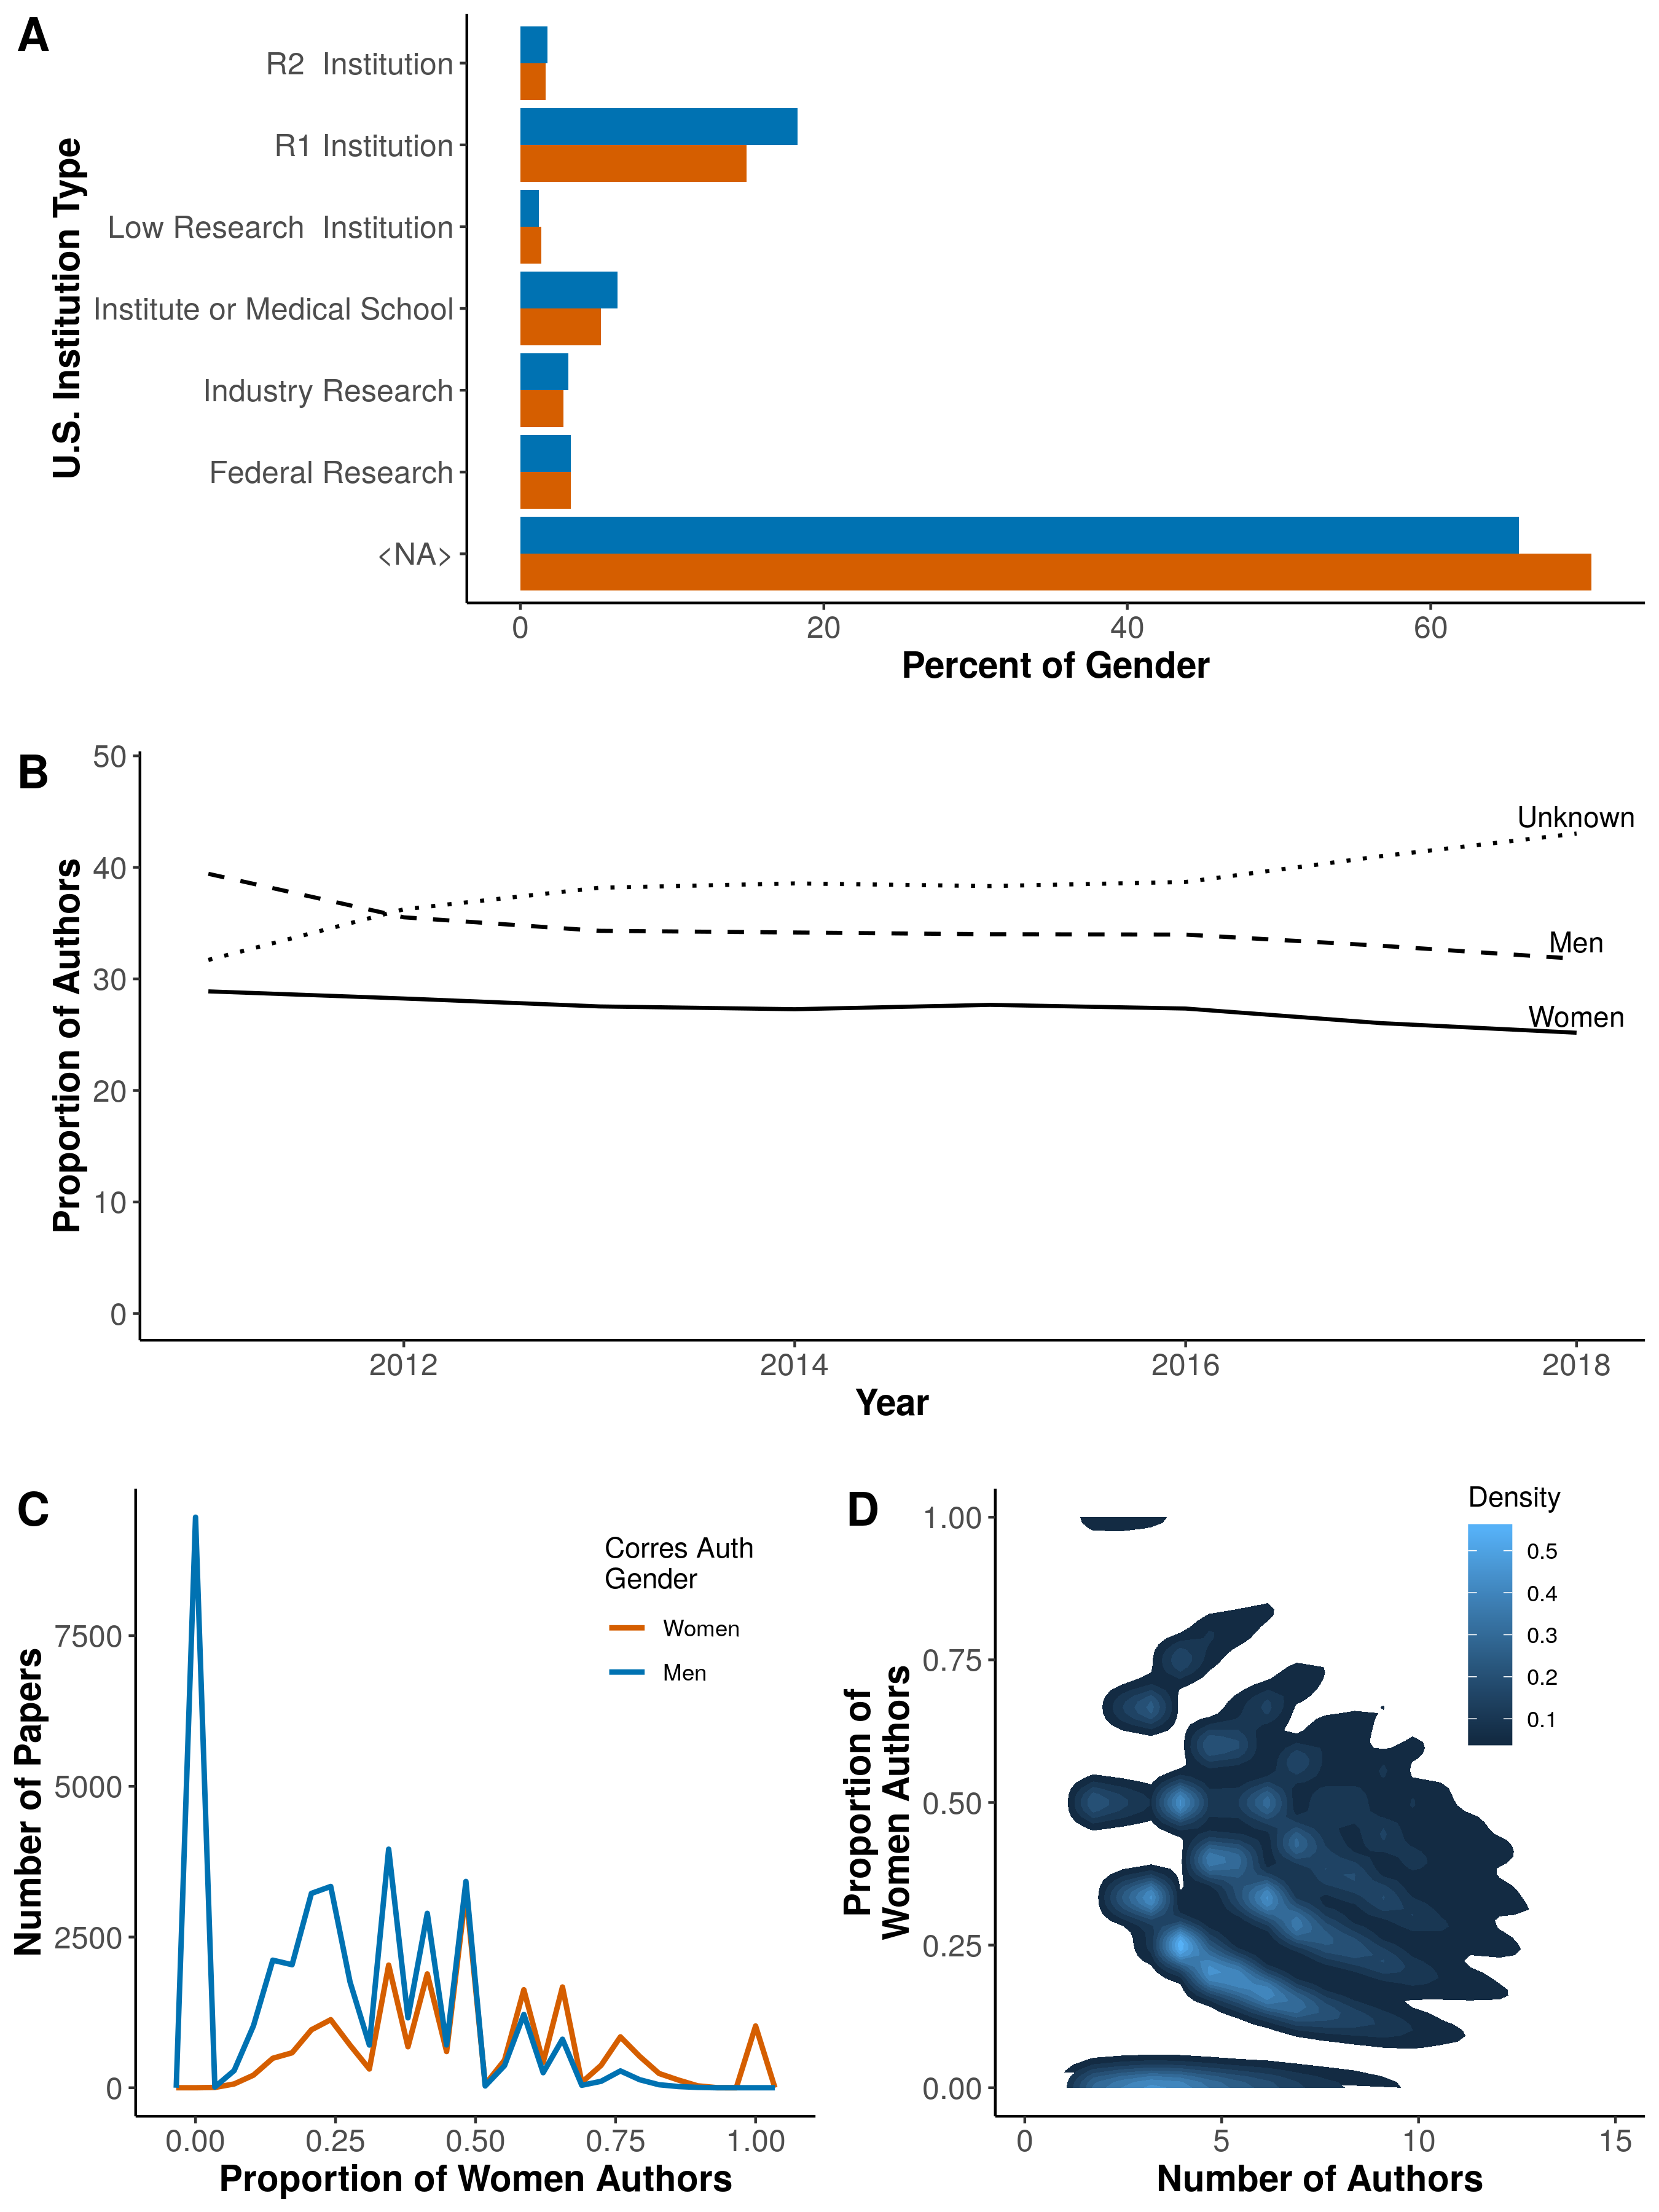
\includegraphics{Figure_3.png} \textbf{Figure 3. Author representation
by gender.} The proportion of (A) men and women authors from each
institution type, (B) men, women, and unknown authors from 2012 - 2018.
Each individual counted once per calendar year. The proportion of (C)
first authors and (D) corresponding authors from 2012 - 2018 on
submitted (dashed) and published (solid) manuscripts.

\newpage

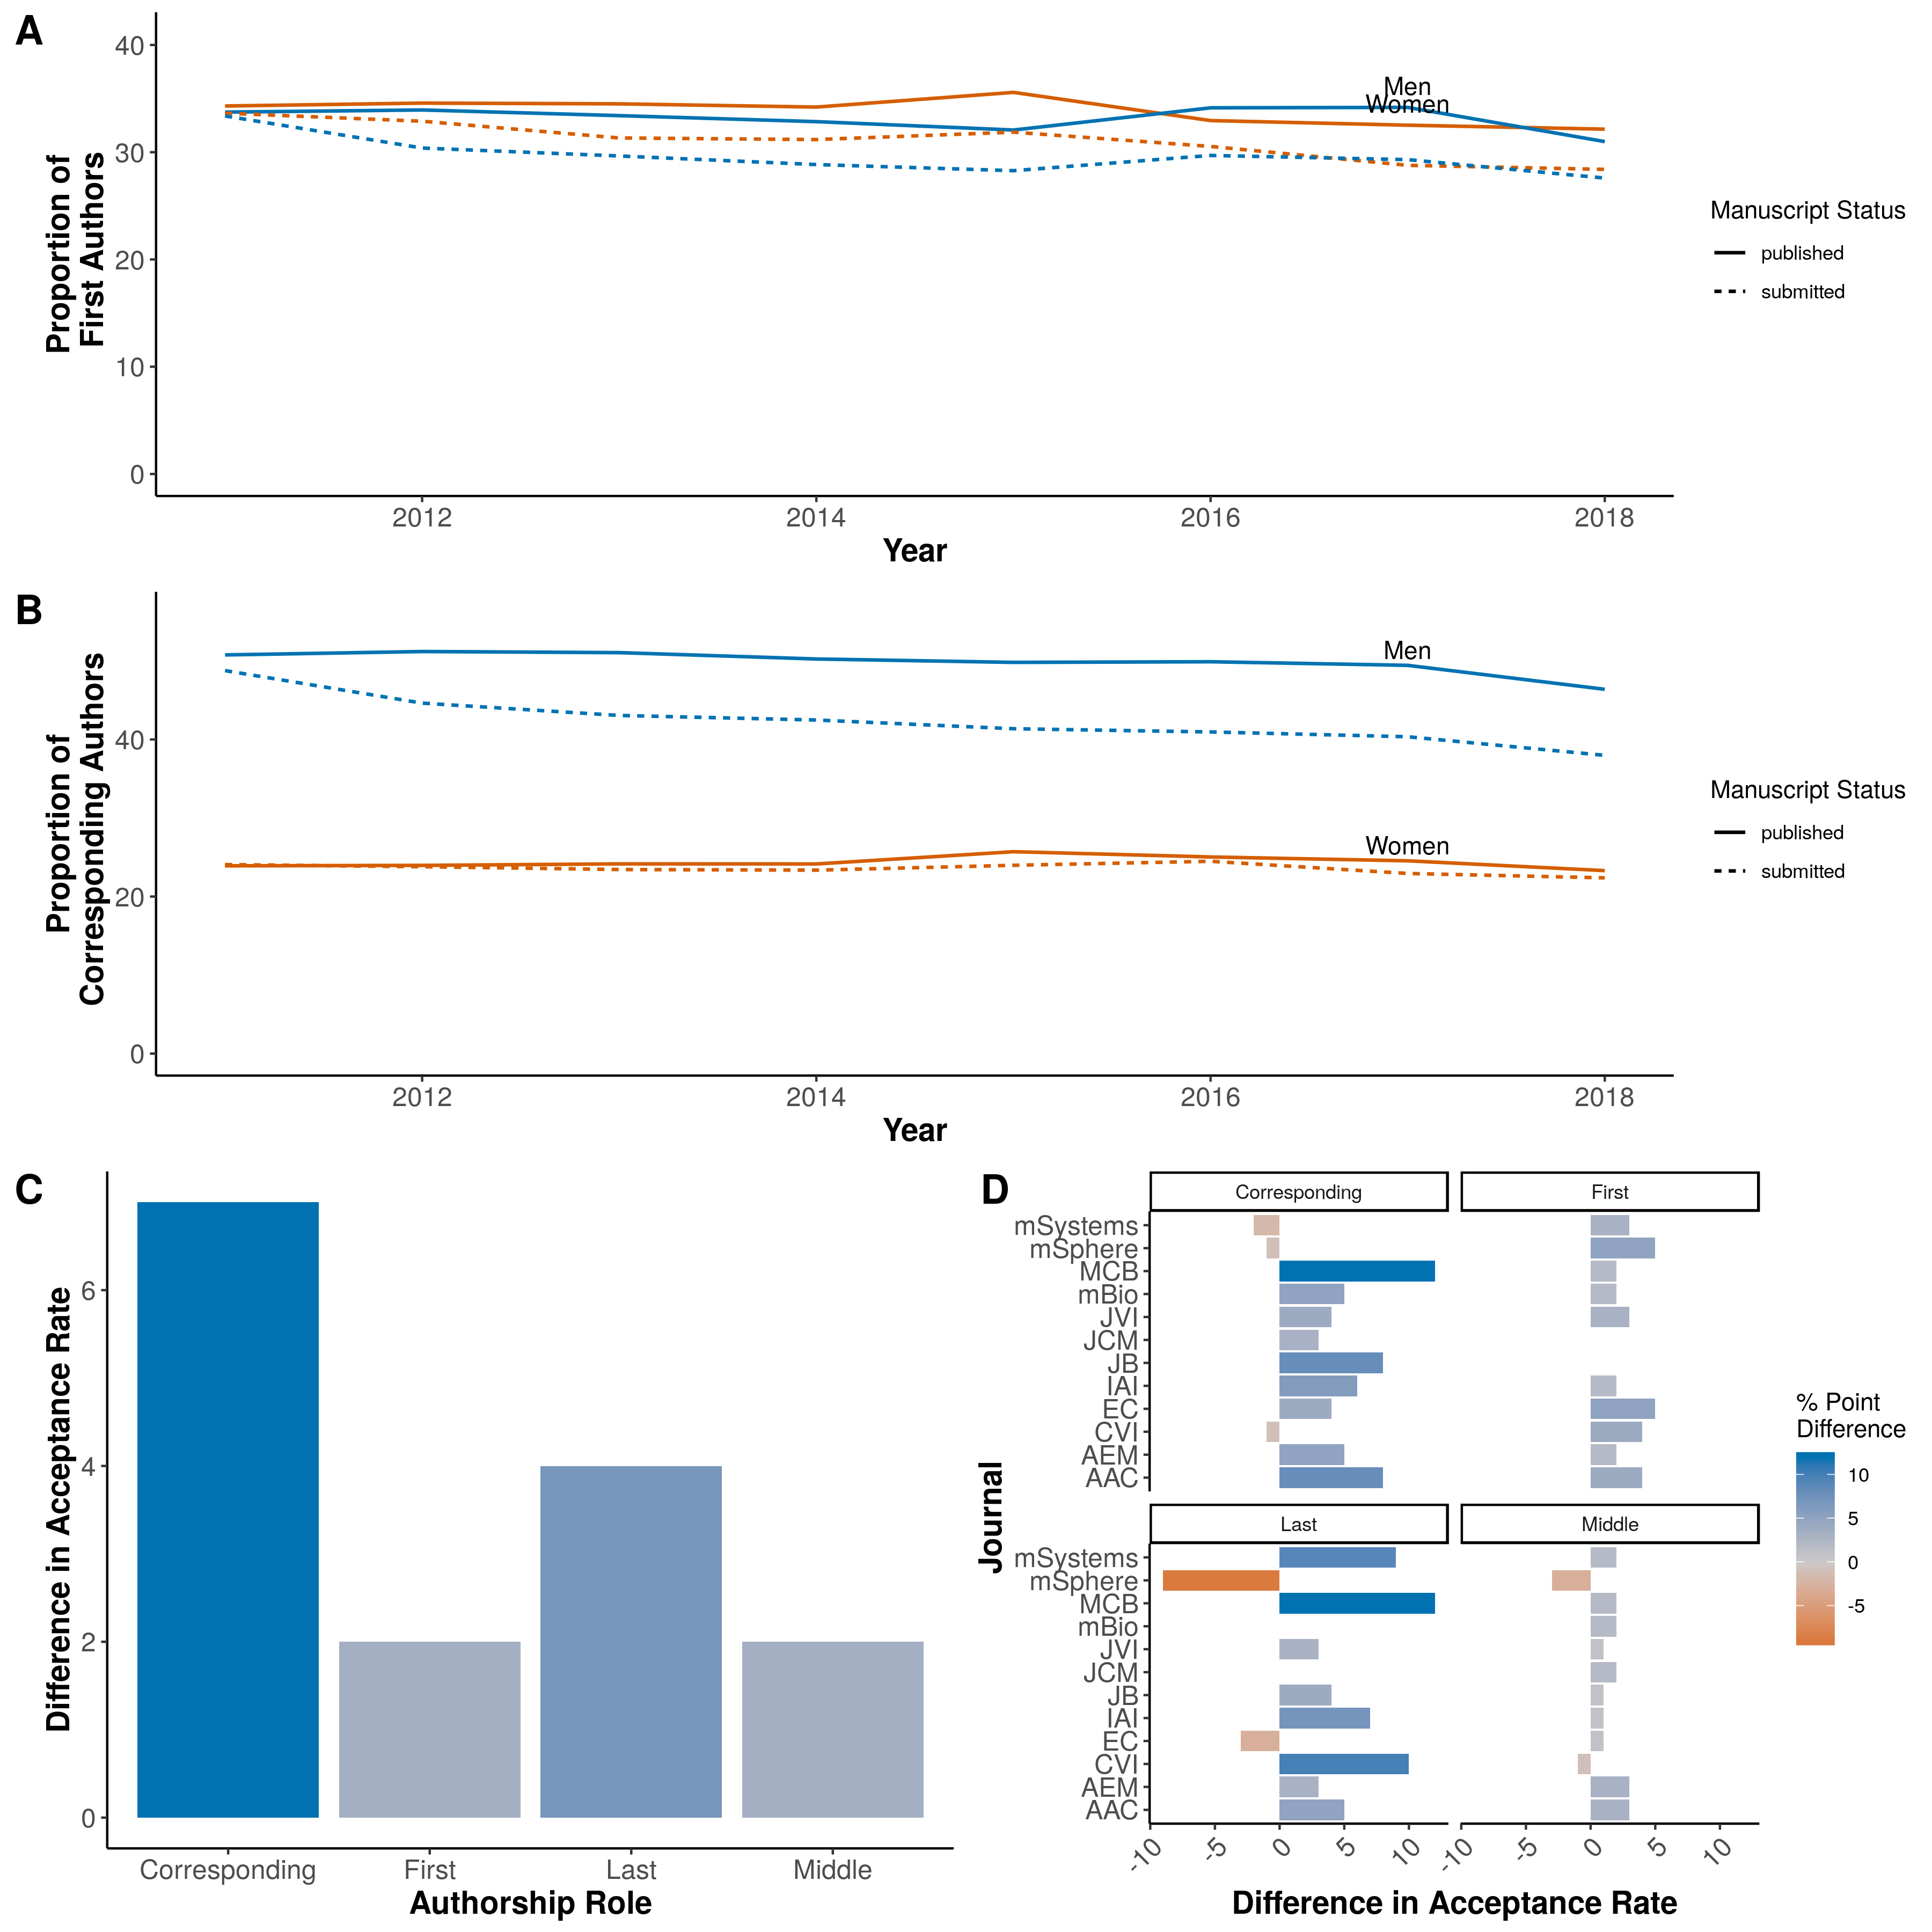
\includegraphics{Figure_4.png} \textbf{Figure 4. Difference in rejection
rates by corresponding author gender.} The percent of manuscripts
rejected by author gender and type (e.g., corresponding, first, last,
middle) at (A) all journals combined. (B) The difference in percent
editorial rejection rates for corresponding authors at each journal,
vertical line indicates the difference for all journals combined. (D)
The difference in percentage points between each decision type for
corresponding authors following the first peer review, vertical lines
indicate the difference value for all journals combined. Absence of a
bar indicates no difference in percentage points.

\newpage

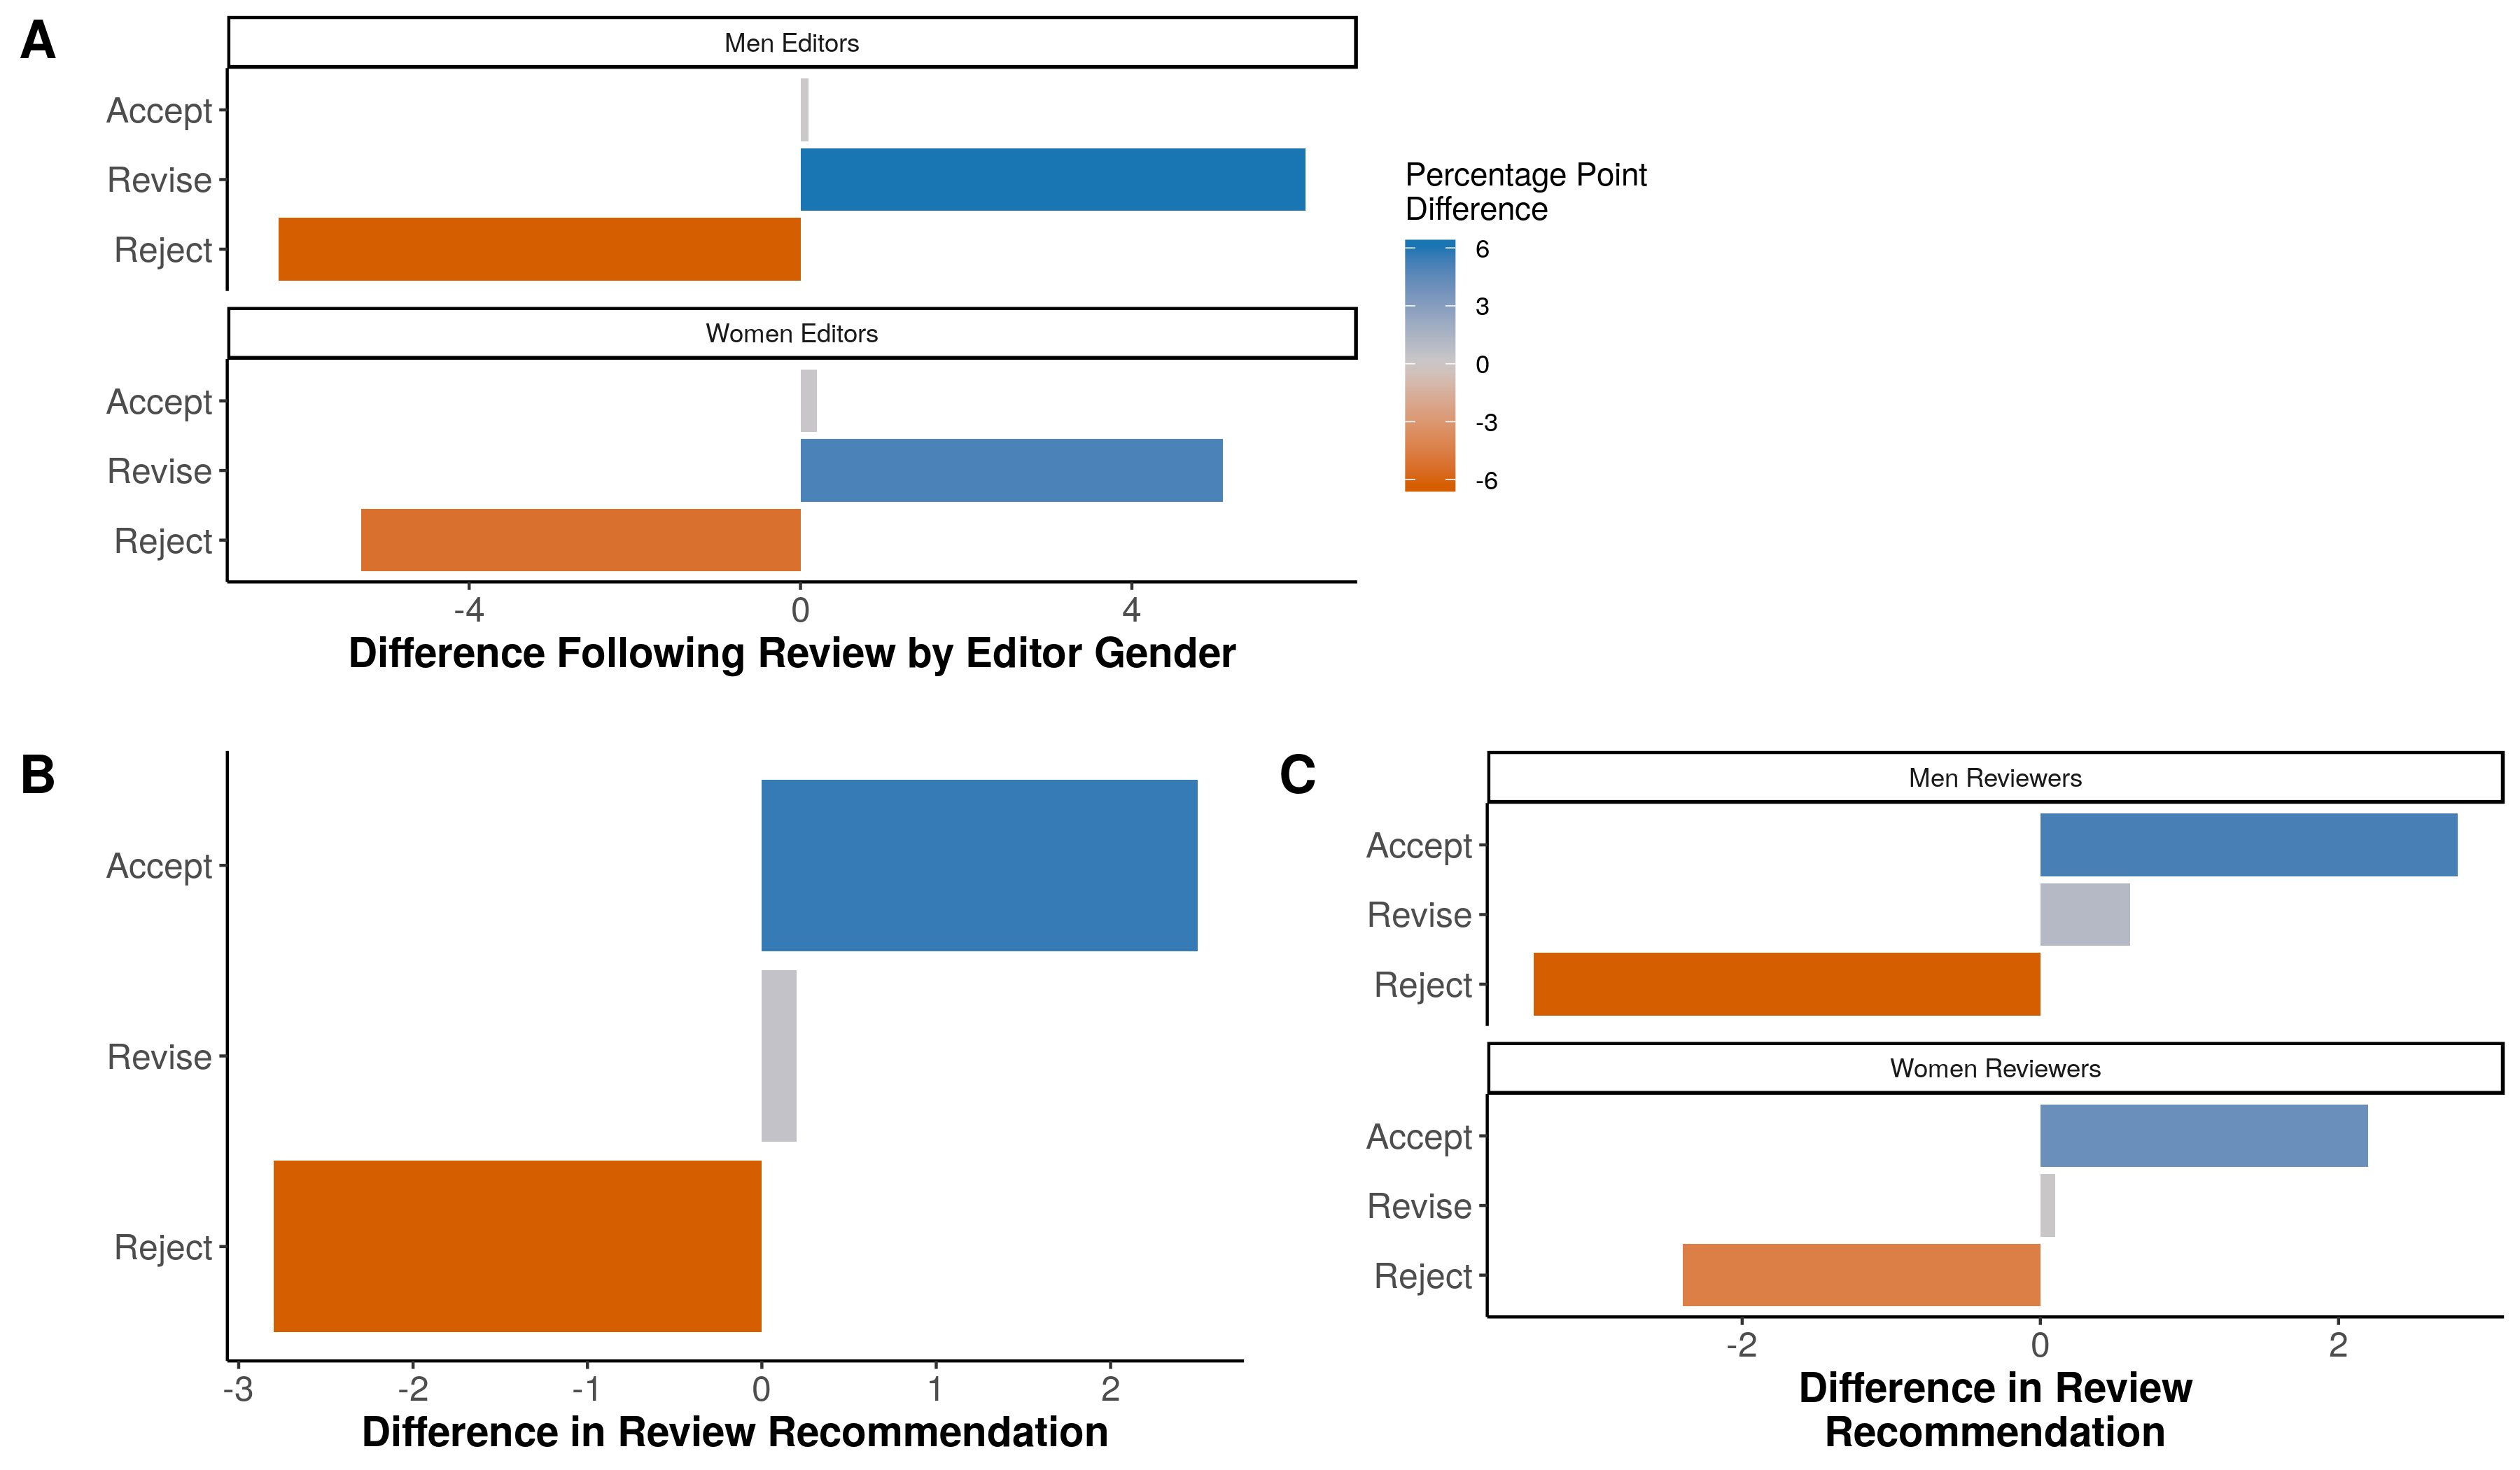
\includegraphics{Figure_5.png} \textbf{Figure 5. Difference in decisions
or recomendations according to the gatekeeper gender.} (A) Effect of
editor gender on the difference in percentage points for decisions
following review at all journals combined. (B) Difference in percentage
points for review recommendations and (C) how that is affected by
reviewer gender.

\newpage

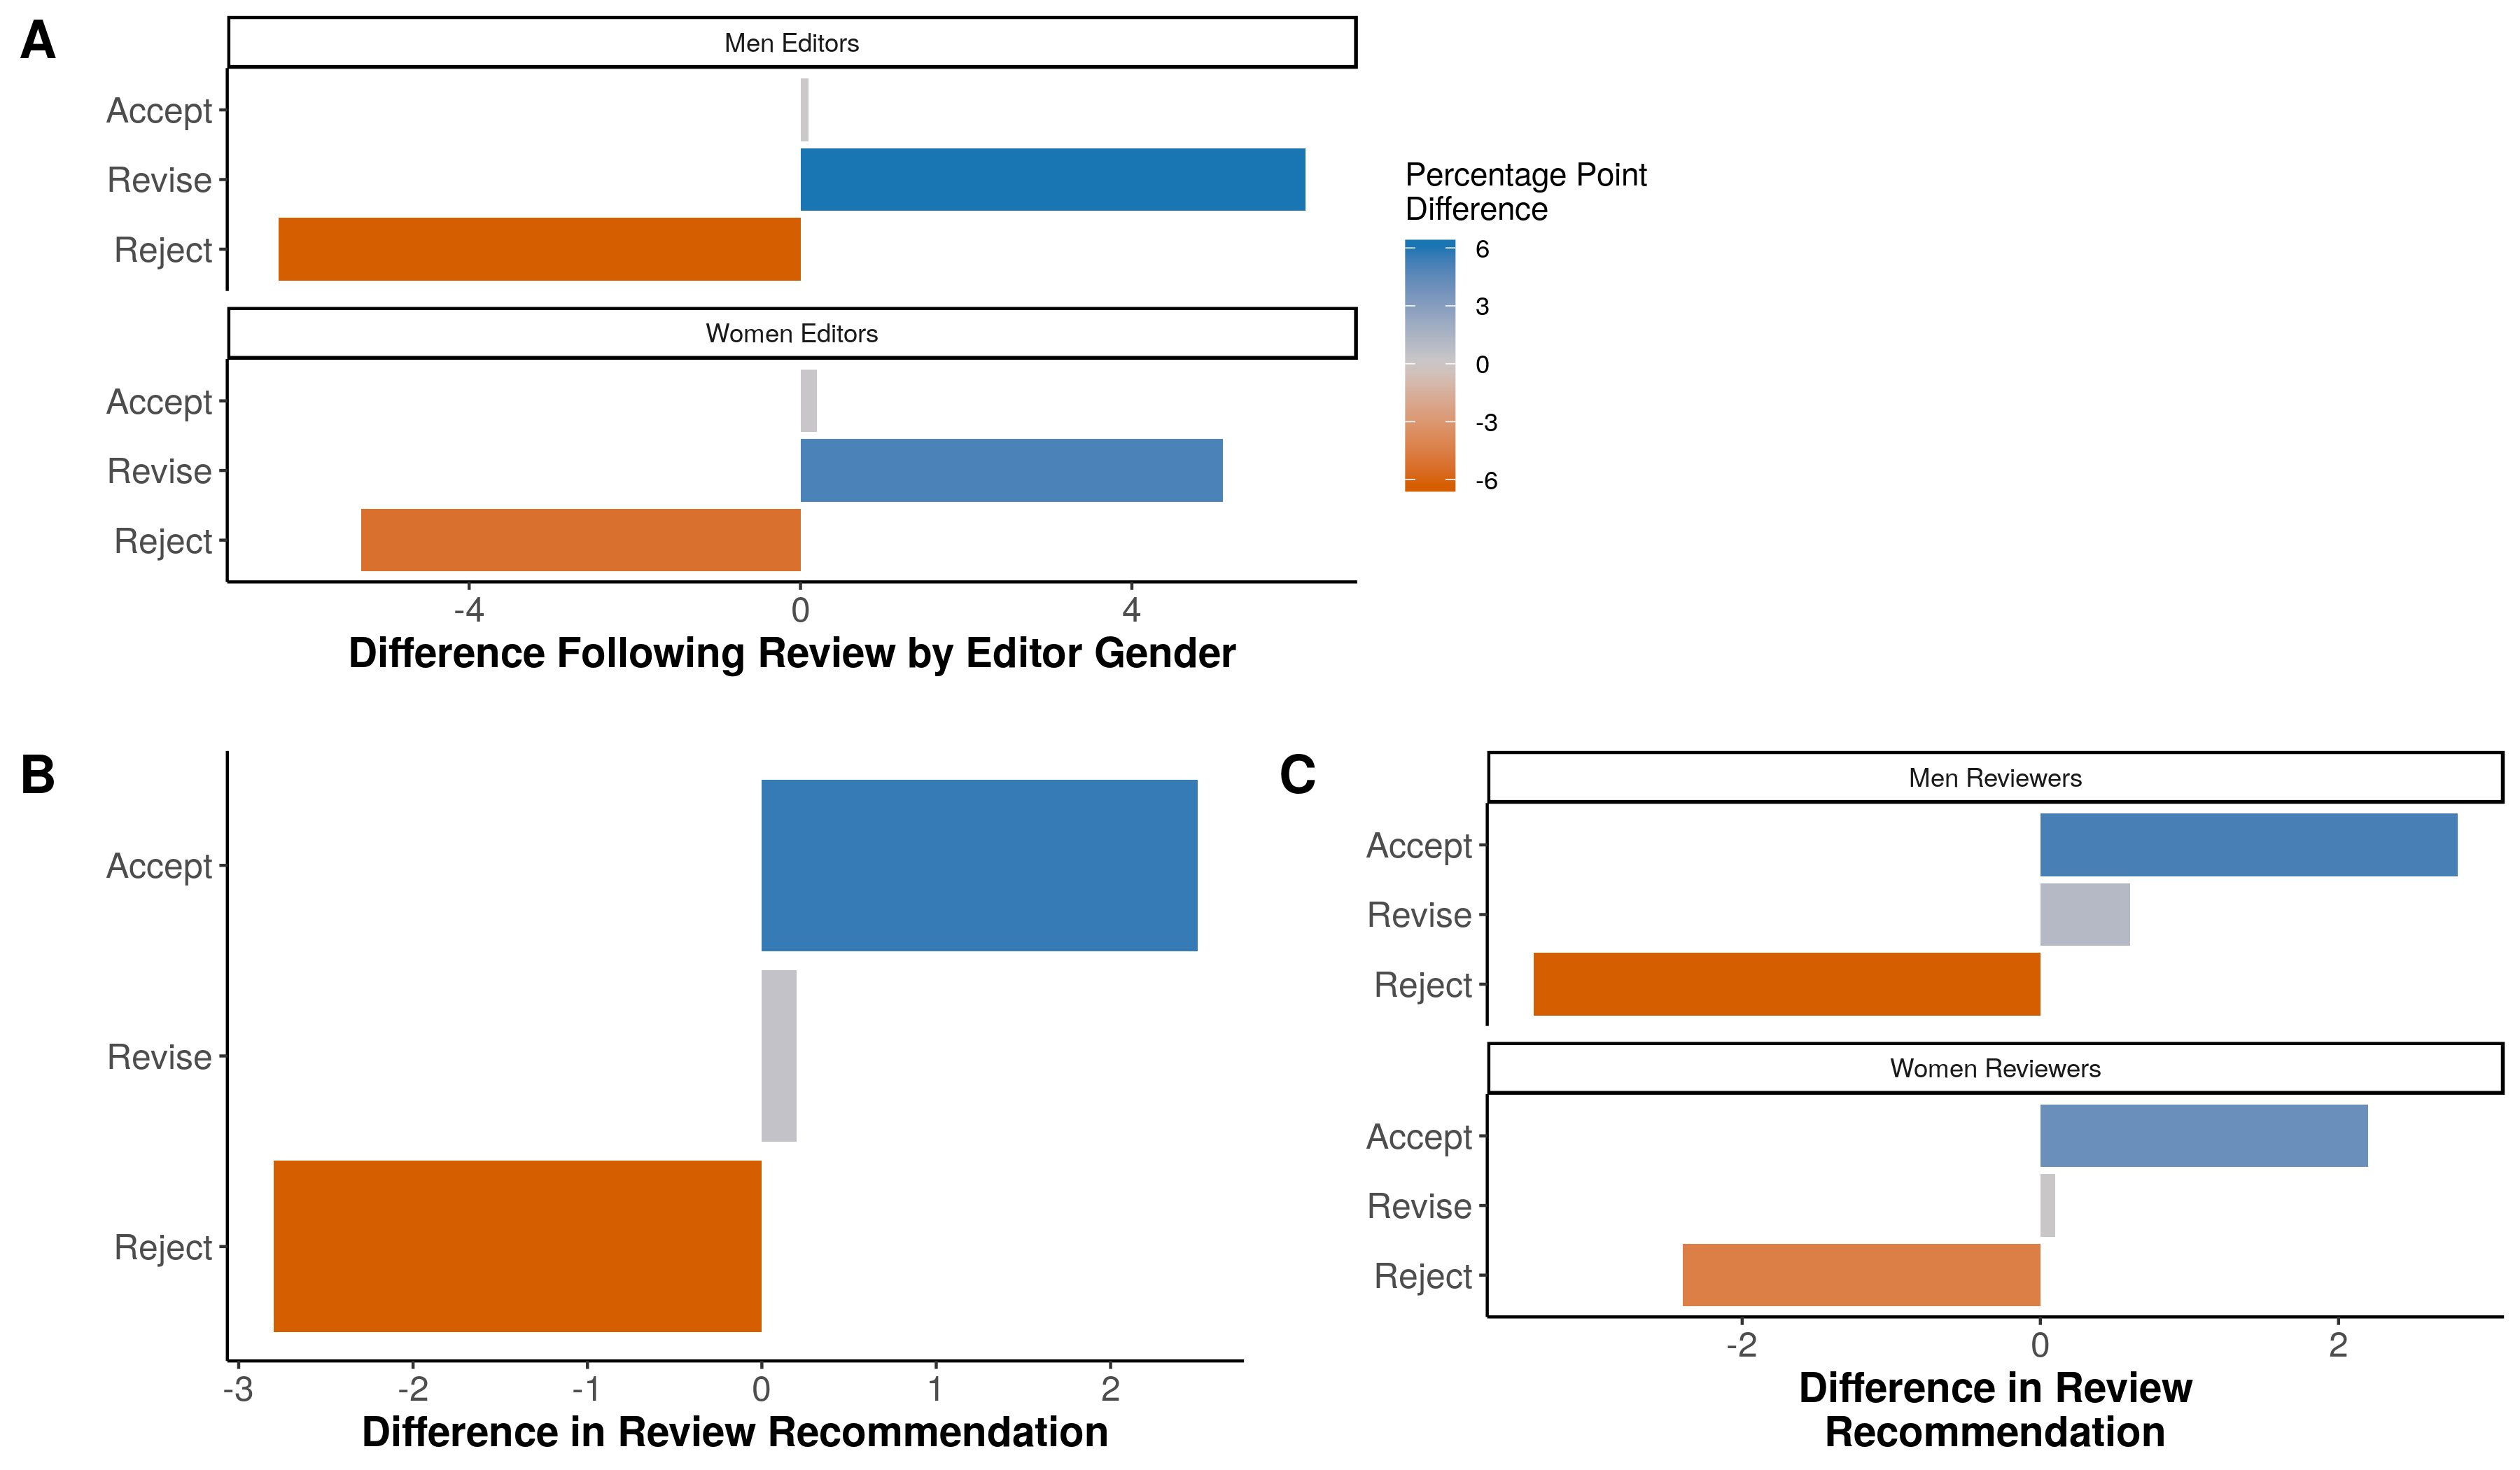
\includegraphics{Figure_6.png} \textbf{Figure 6. Impact of origin and
U.S. institution type on manuscript decisions by gender.} Difference in
percentage points for (A) editorial rejections and (B) following first
review of manuscripts submitted by US-based corresponding authors.
Vertical line indicates value for all ASM journals combined. (C)
Difference in percentage points for acceptance and editorial rejections
according to institution types and (D) acceptance decisions by to editor
gender and institution types.

\newpage

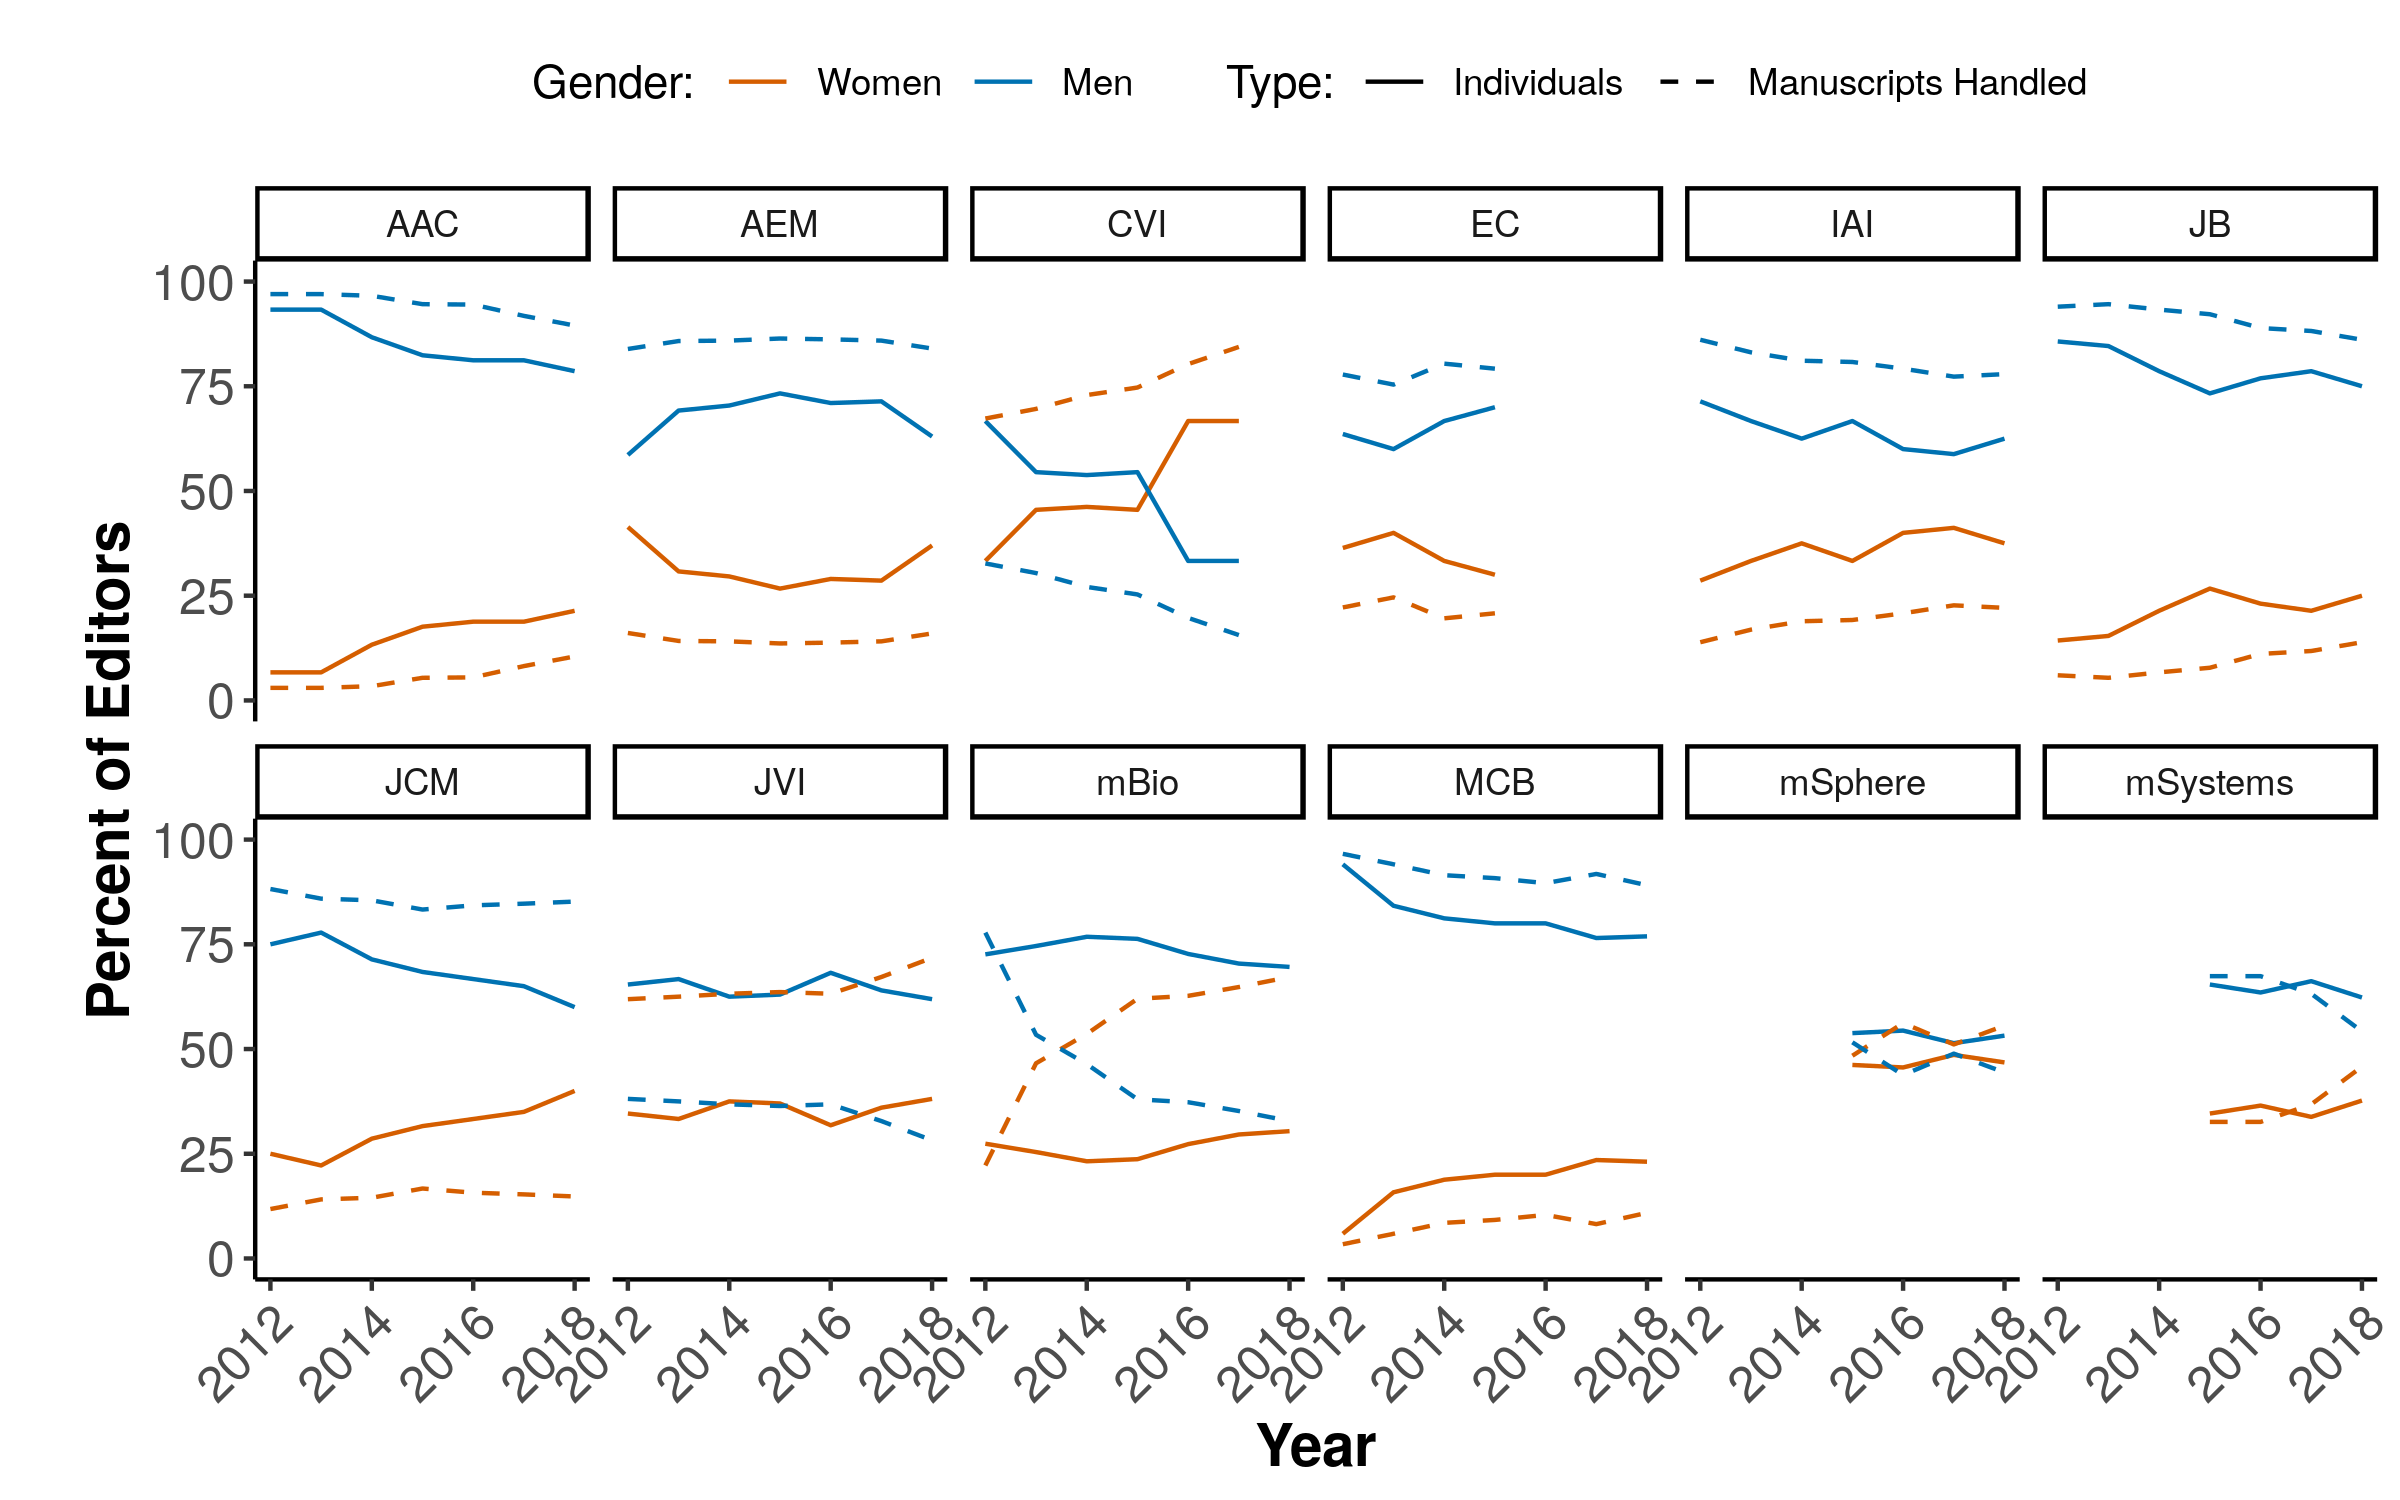
\includegraphics{Figure_S1.png} Figure S1. The proportion of editors
(solid line) and their workloads (dashed line) at each ASM journal from
2012 to 2018.

\newpage

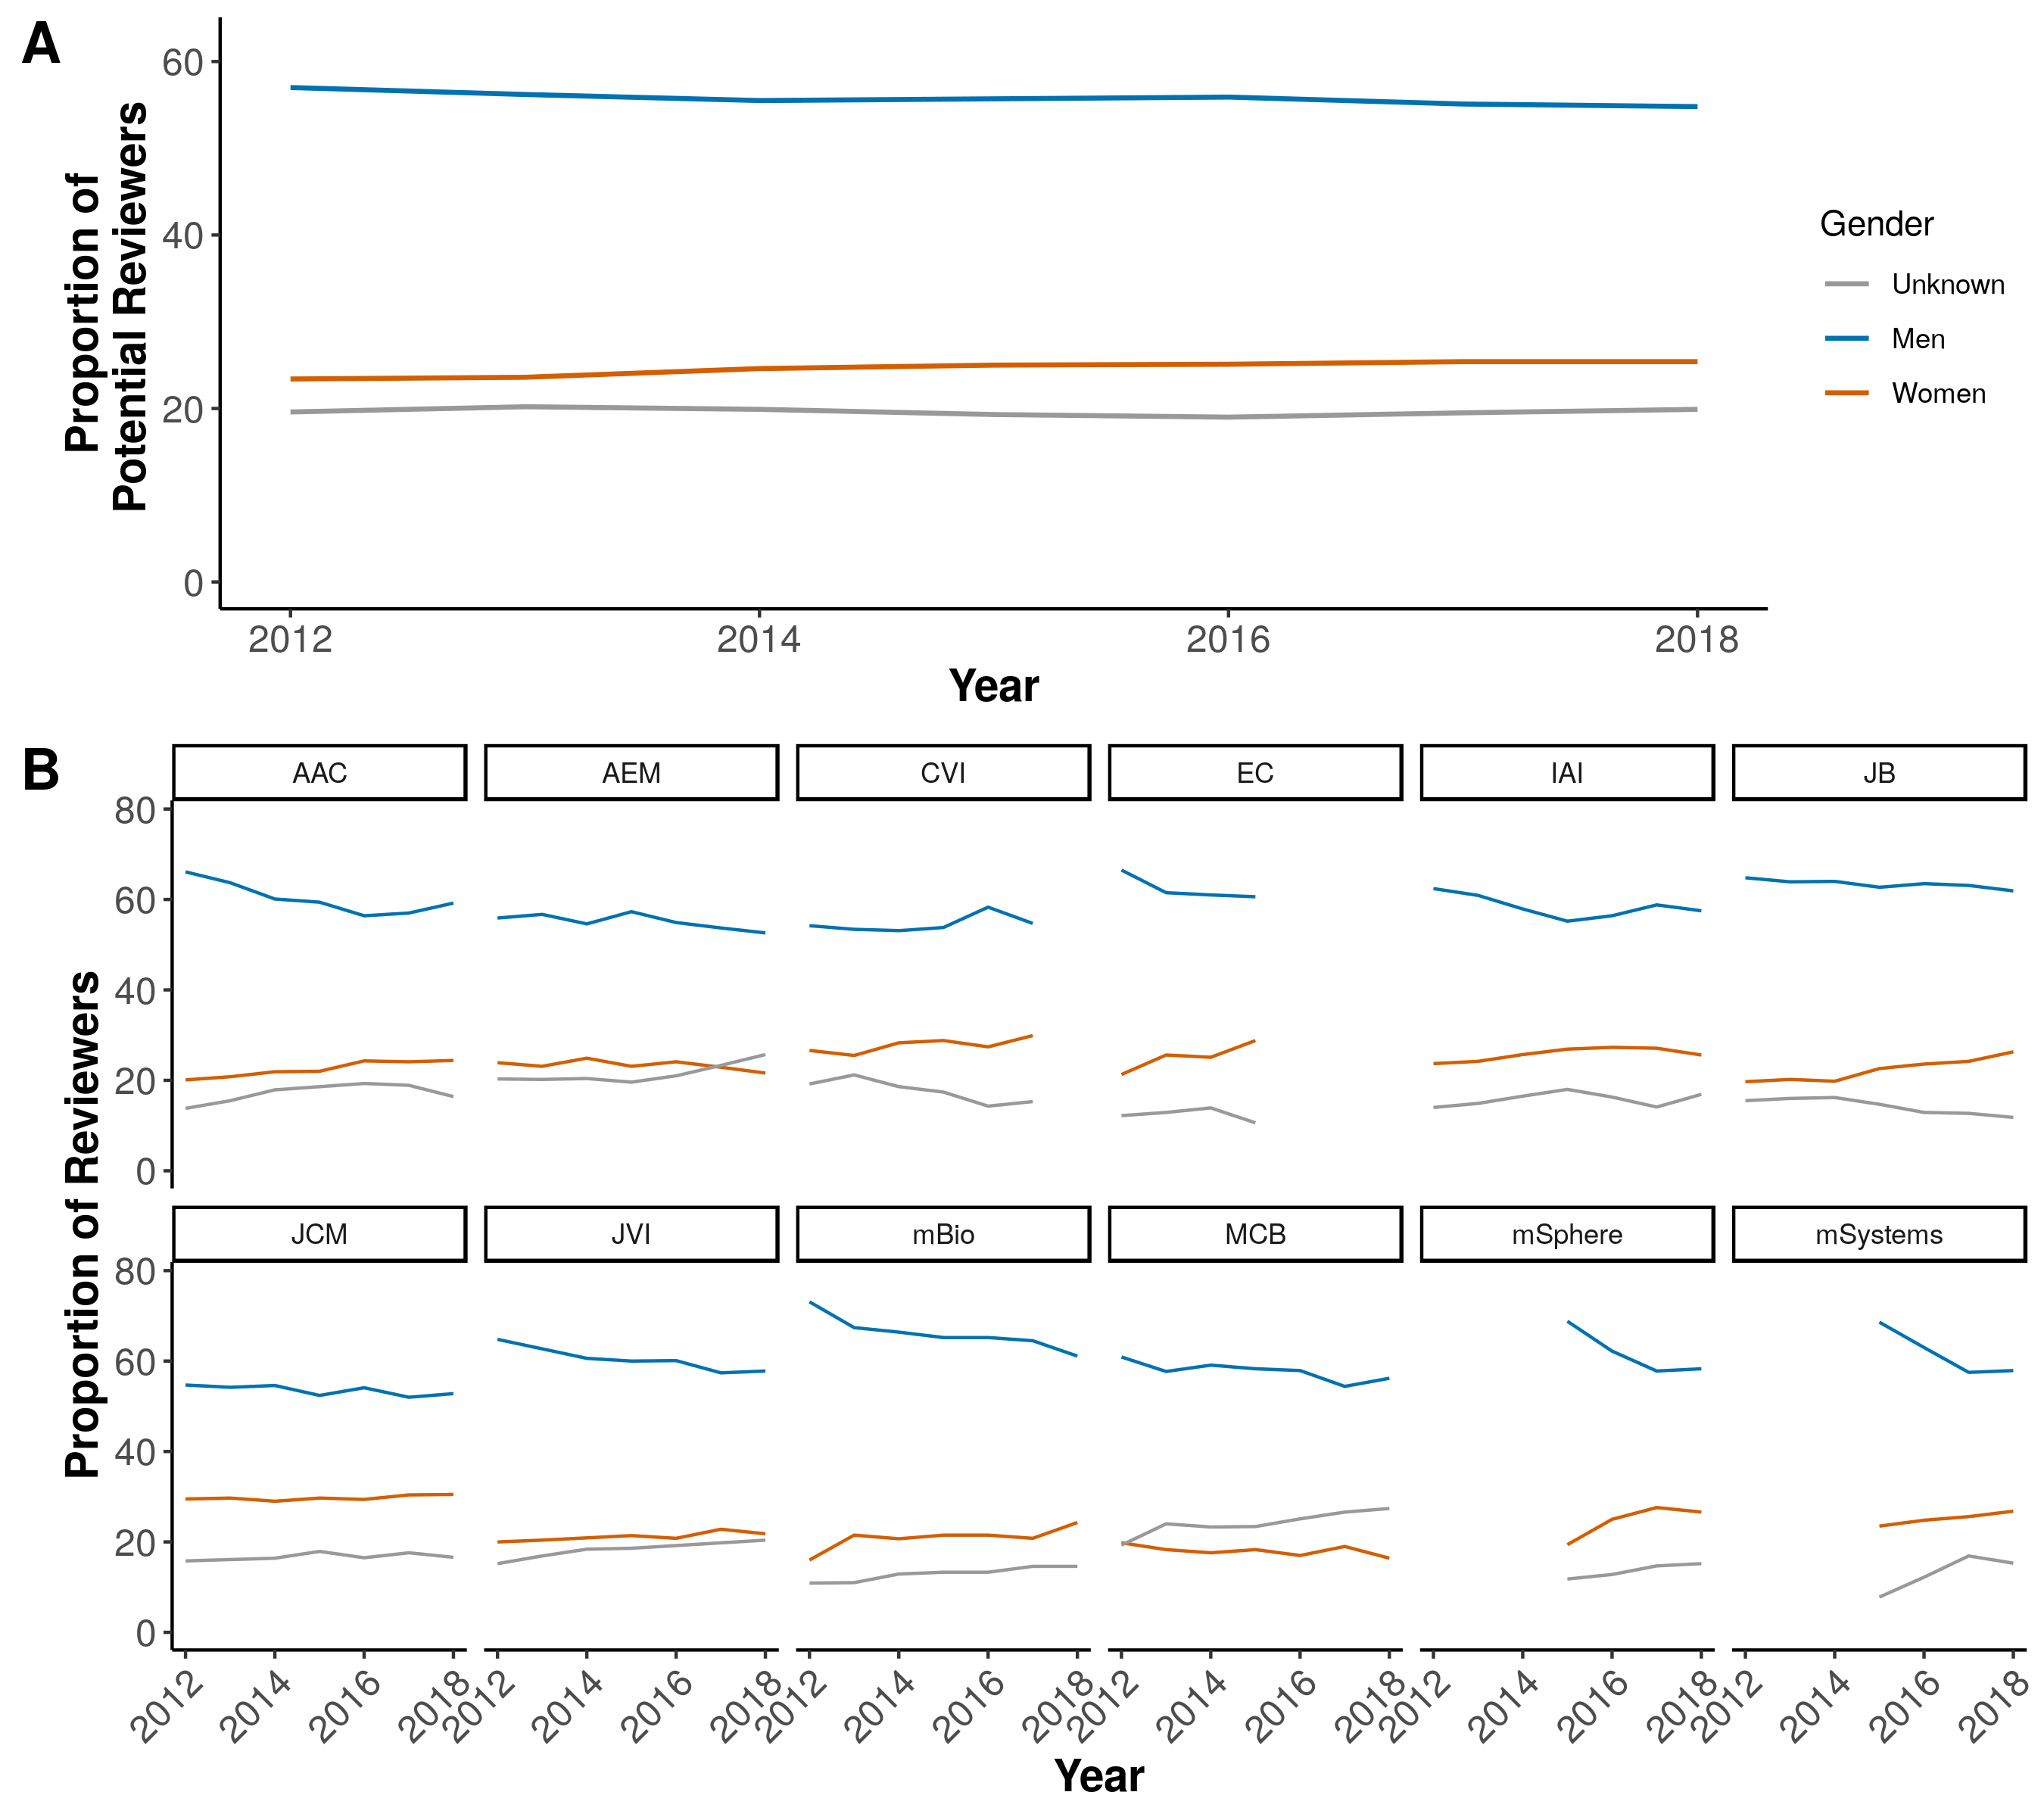
\includegraphics{Figure_S2.png} Figure S2. The proportion of (A)
potential reviewers at all ASM journals combined, (B) reviewers at each
ASM journal.

\newpage

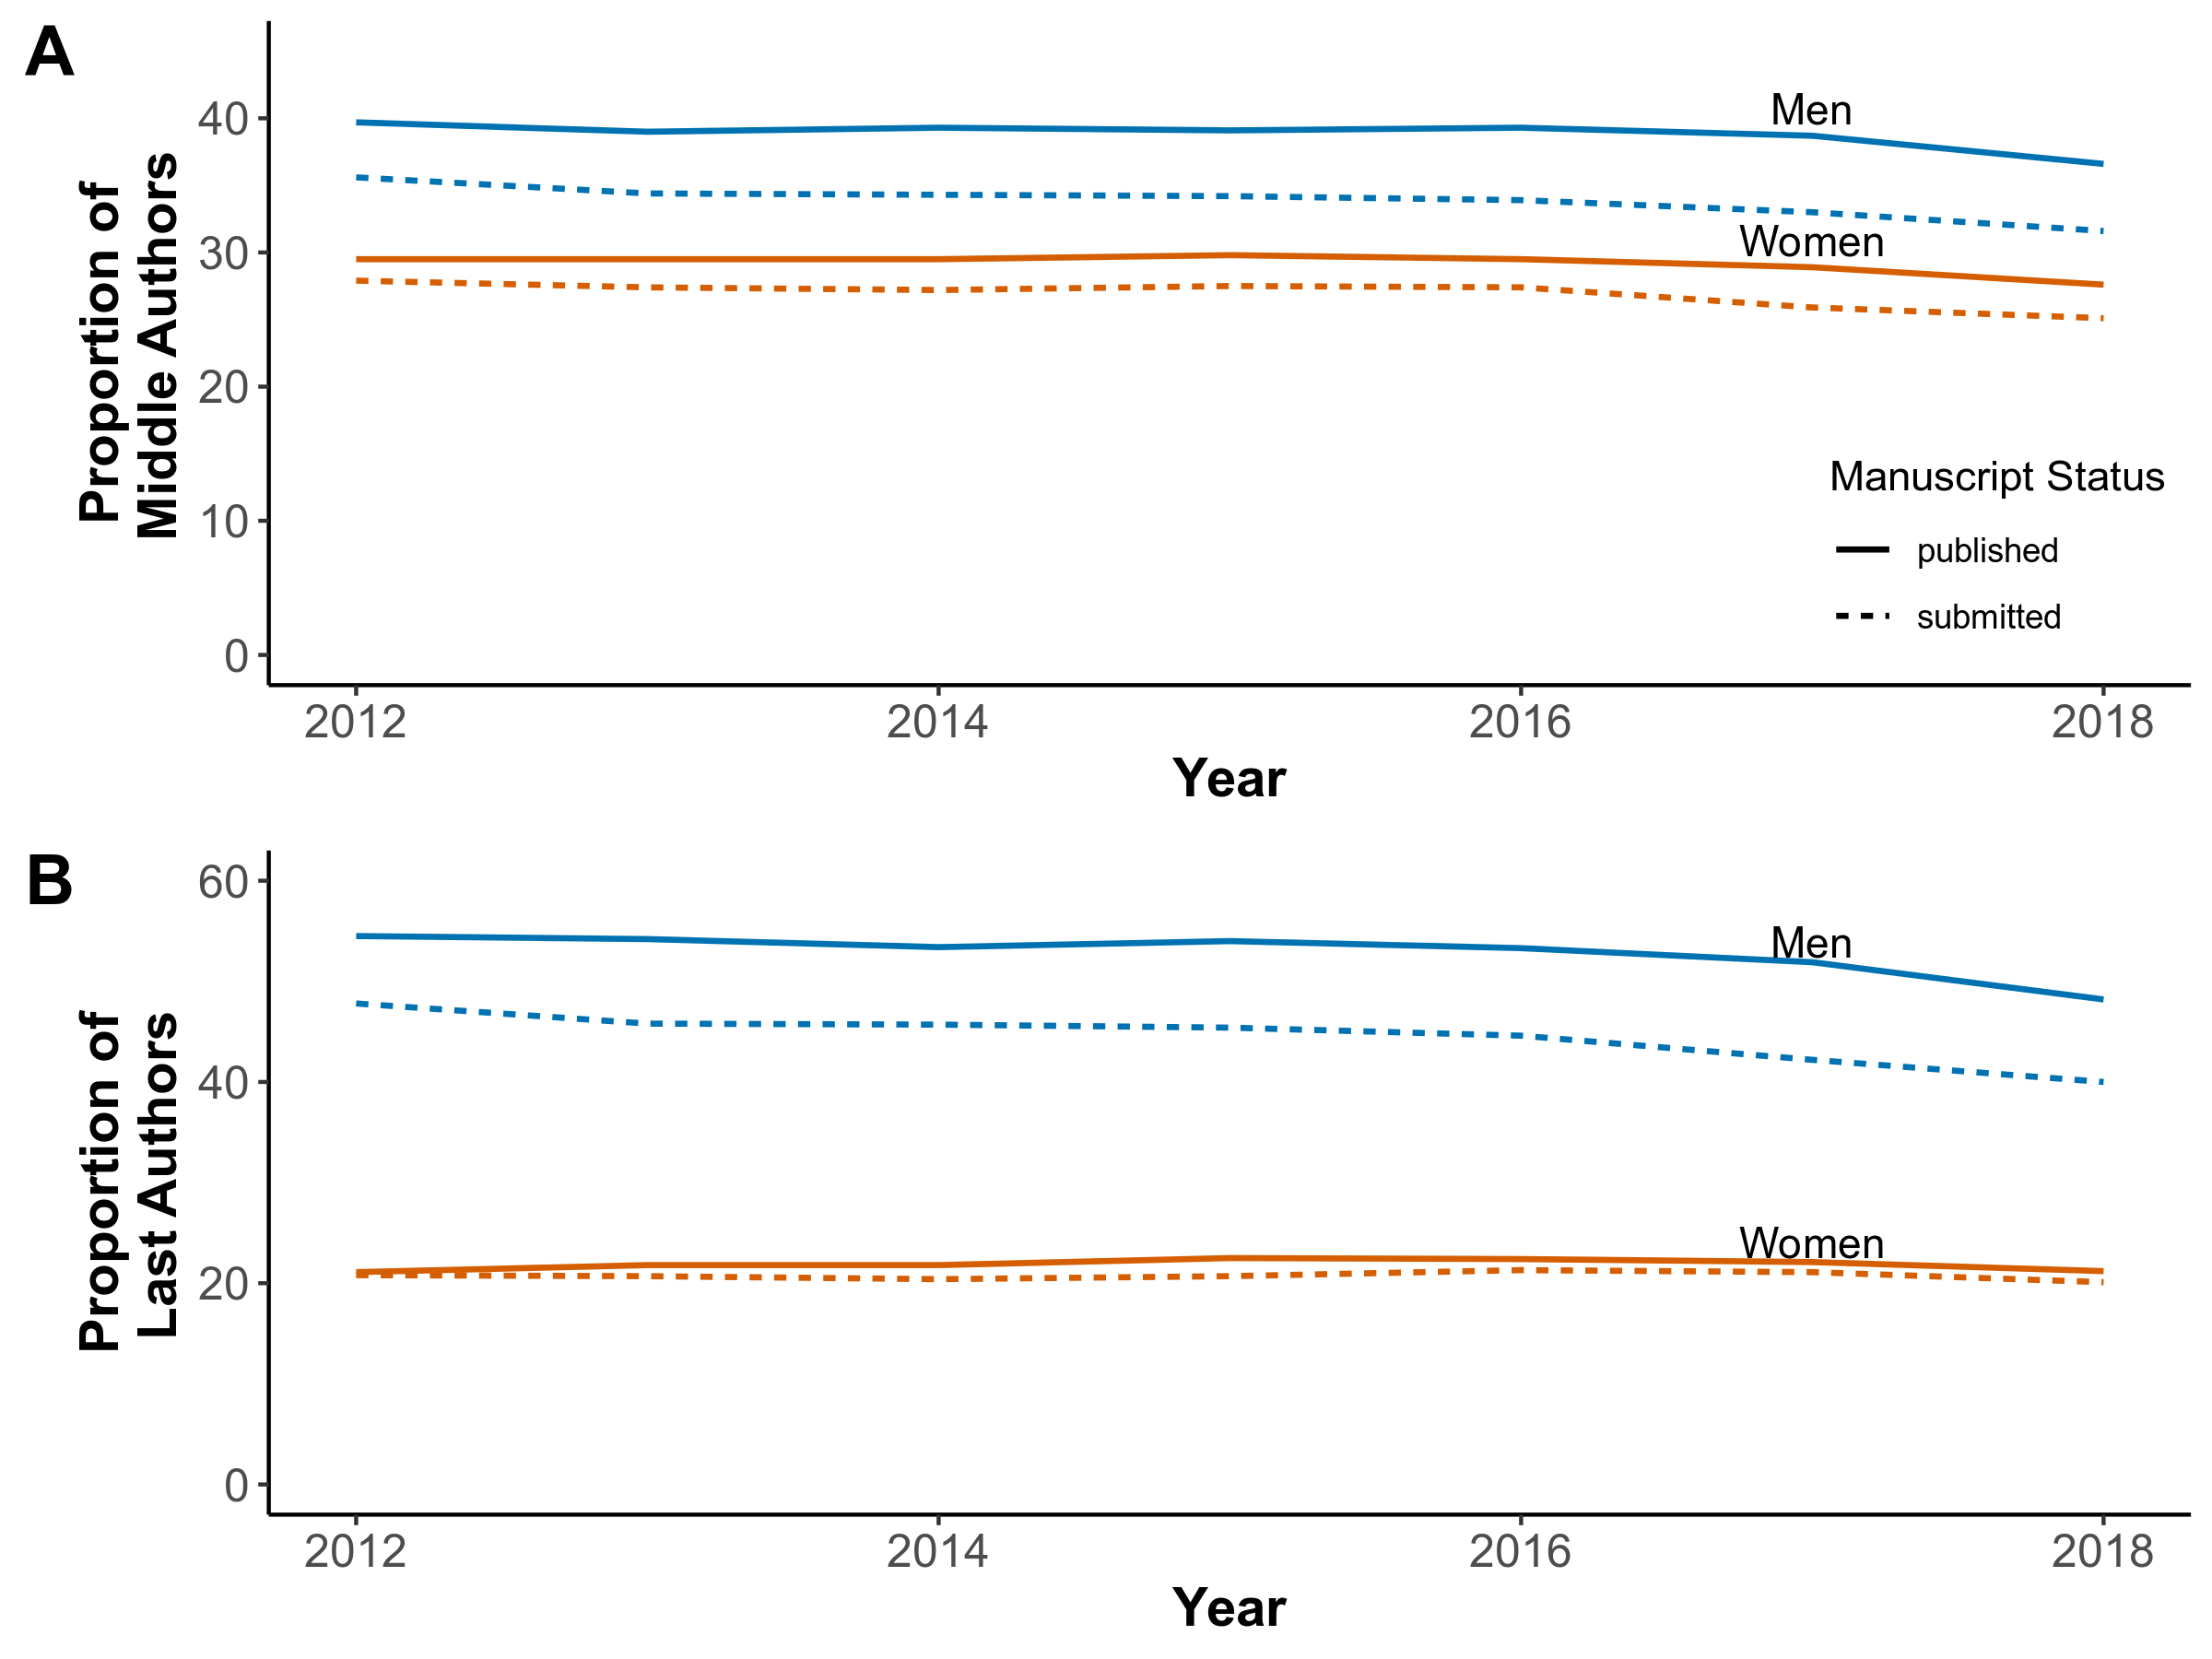
\includegraphics{Figure_S3.png} Figure S3. The proportion of all
submitting (dashed line) and publishing (solid line) (A) middle and (B)
last authors by gender at each ASM journal.

\newpage

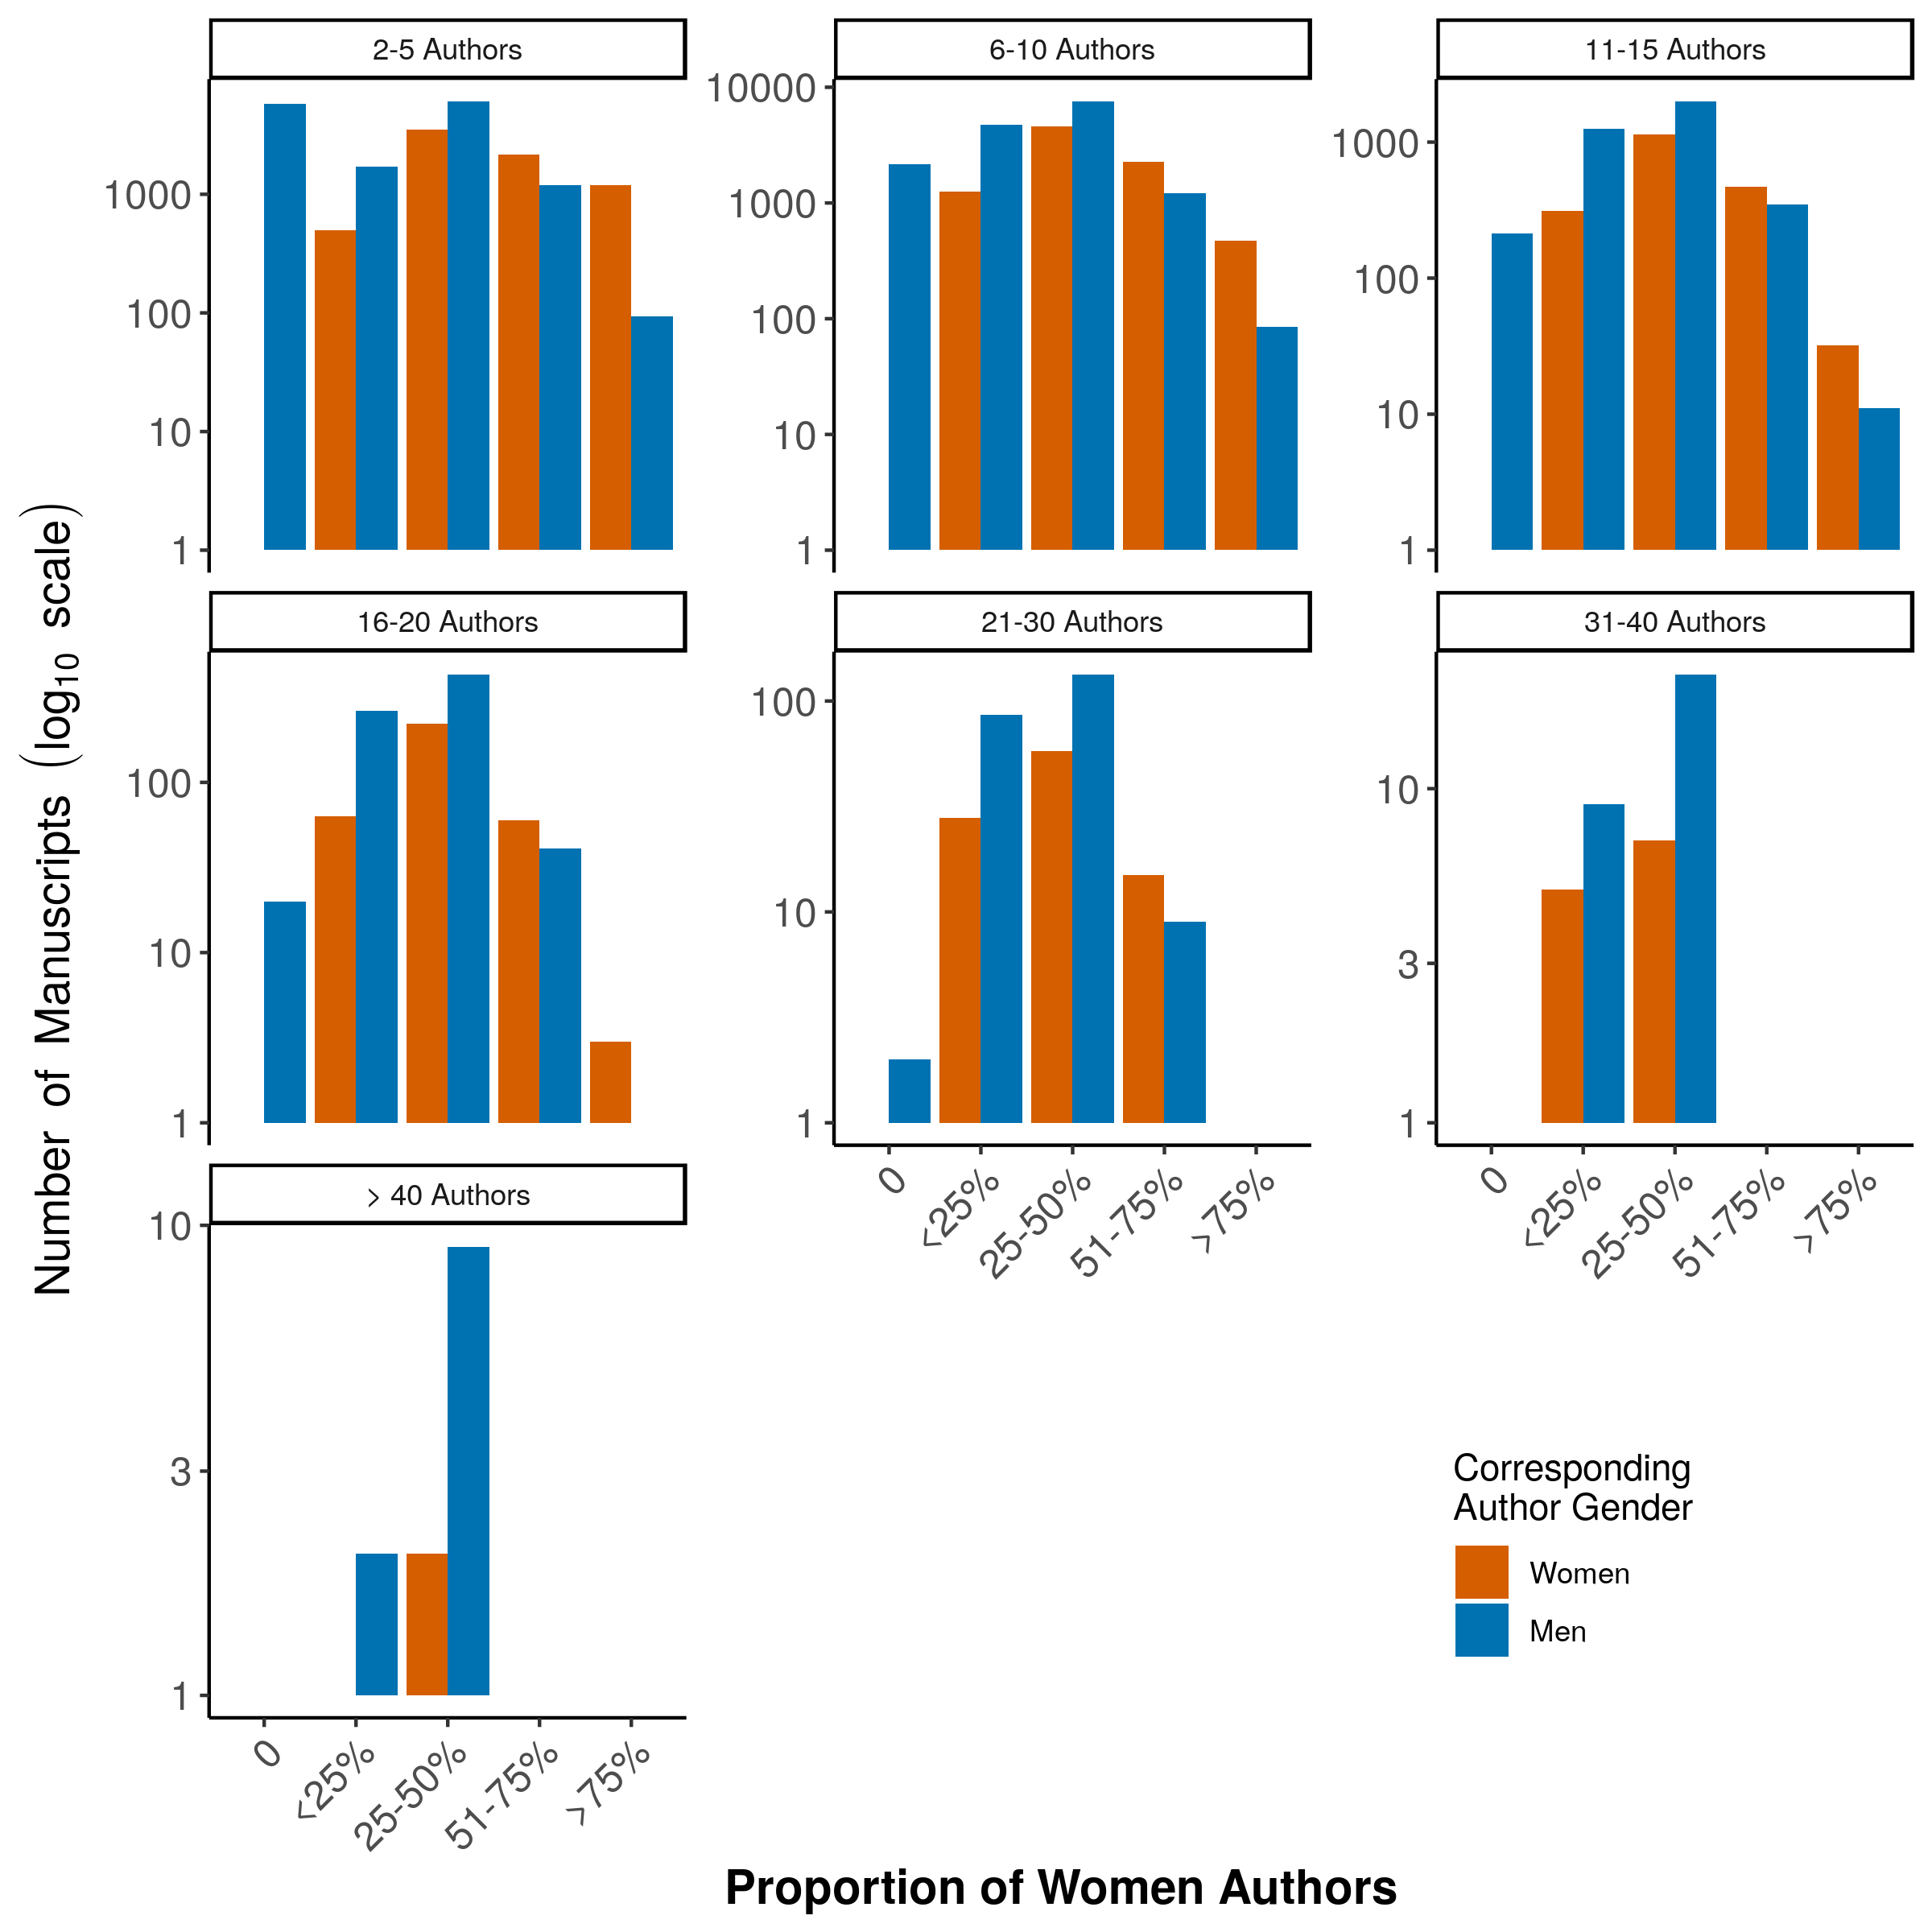
\includegraphics{Figure_S4.png} Figure S4. The proportion of women
authors on submitted manuscripts according to the number of authors and
the gender of the corresponding author.

\newpage

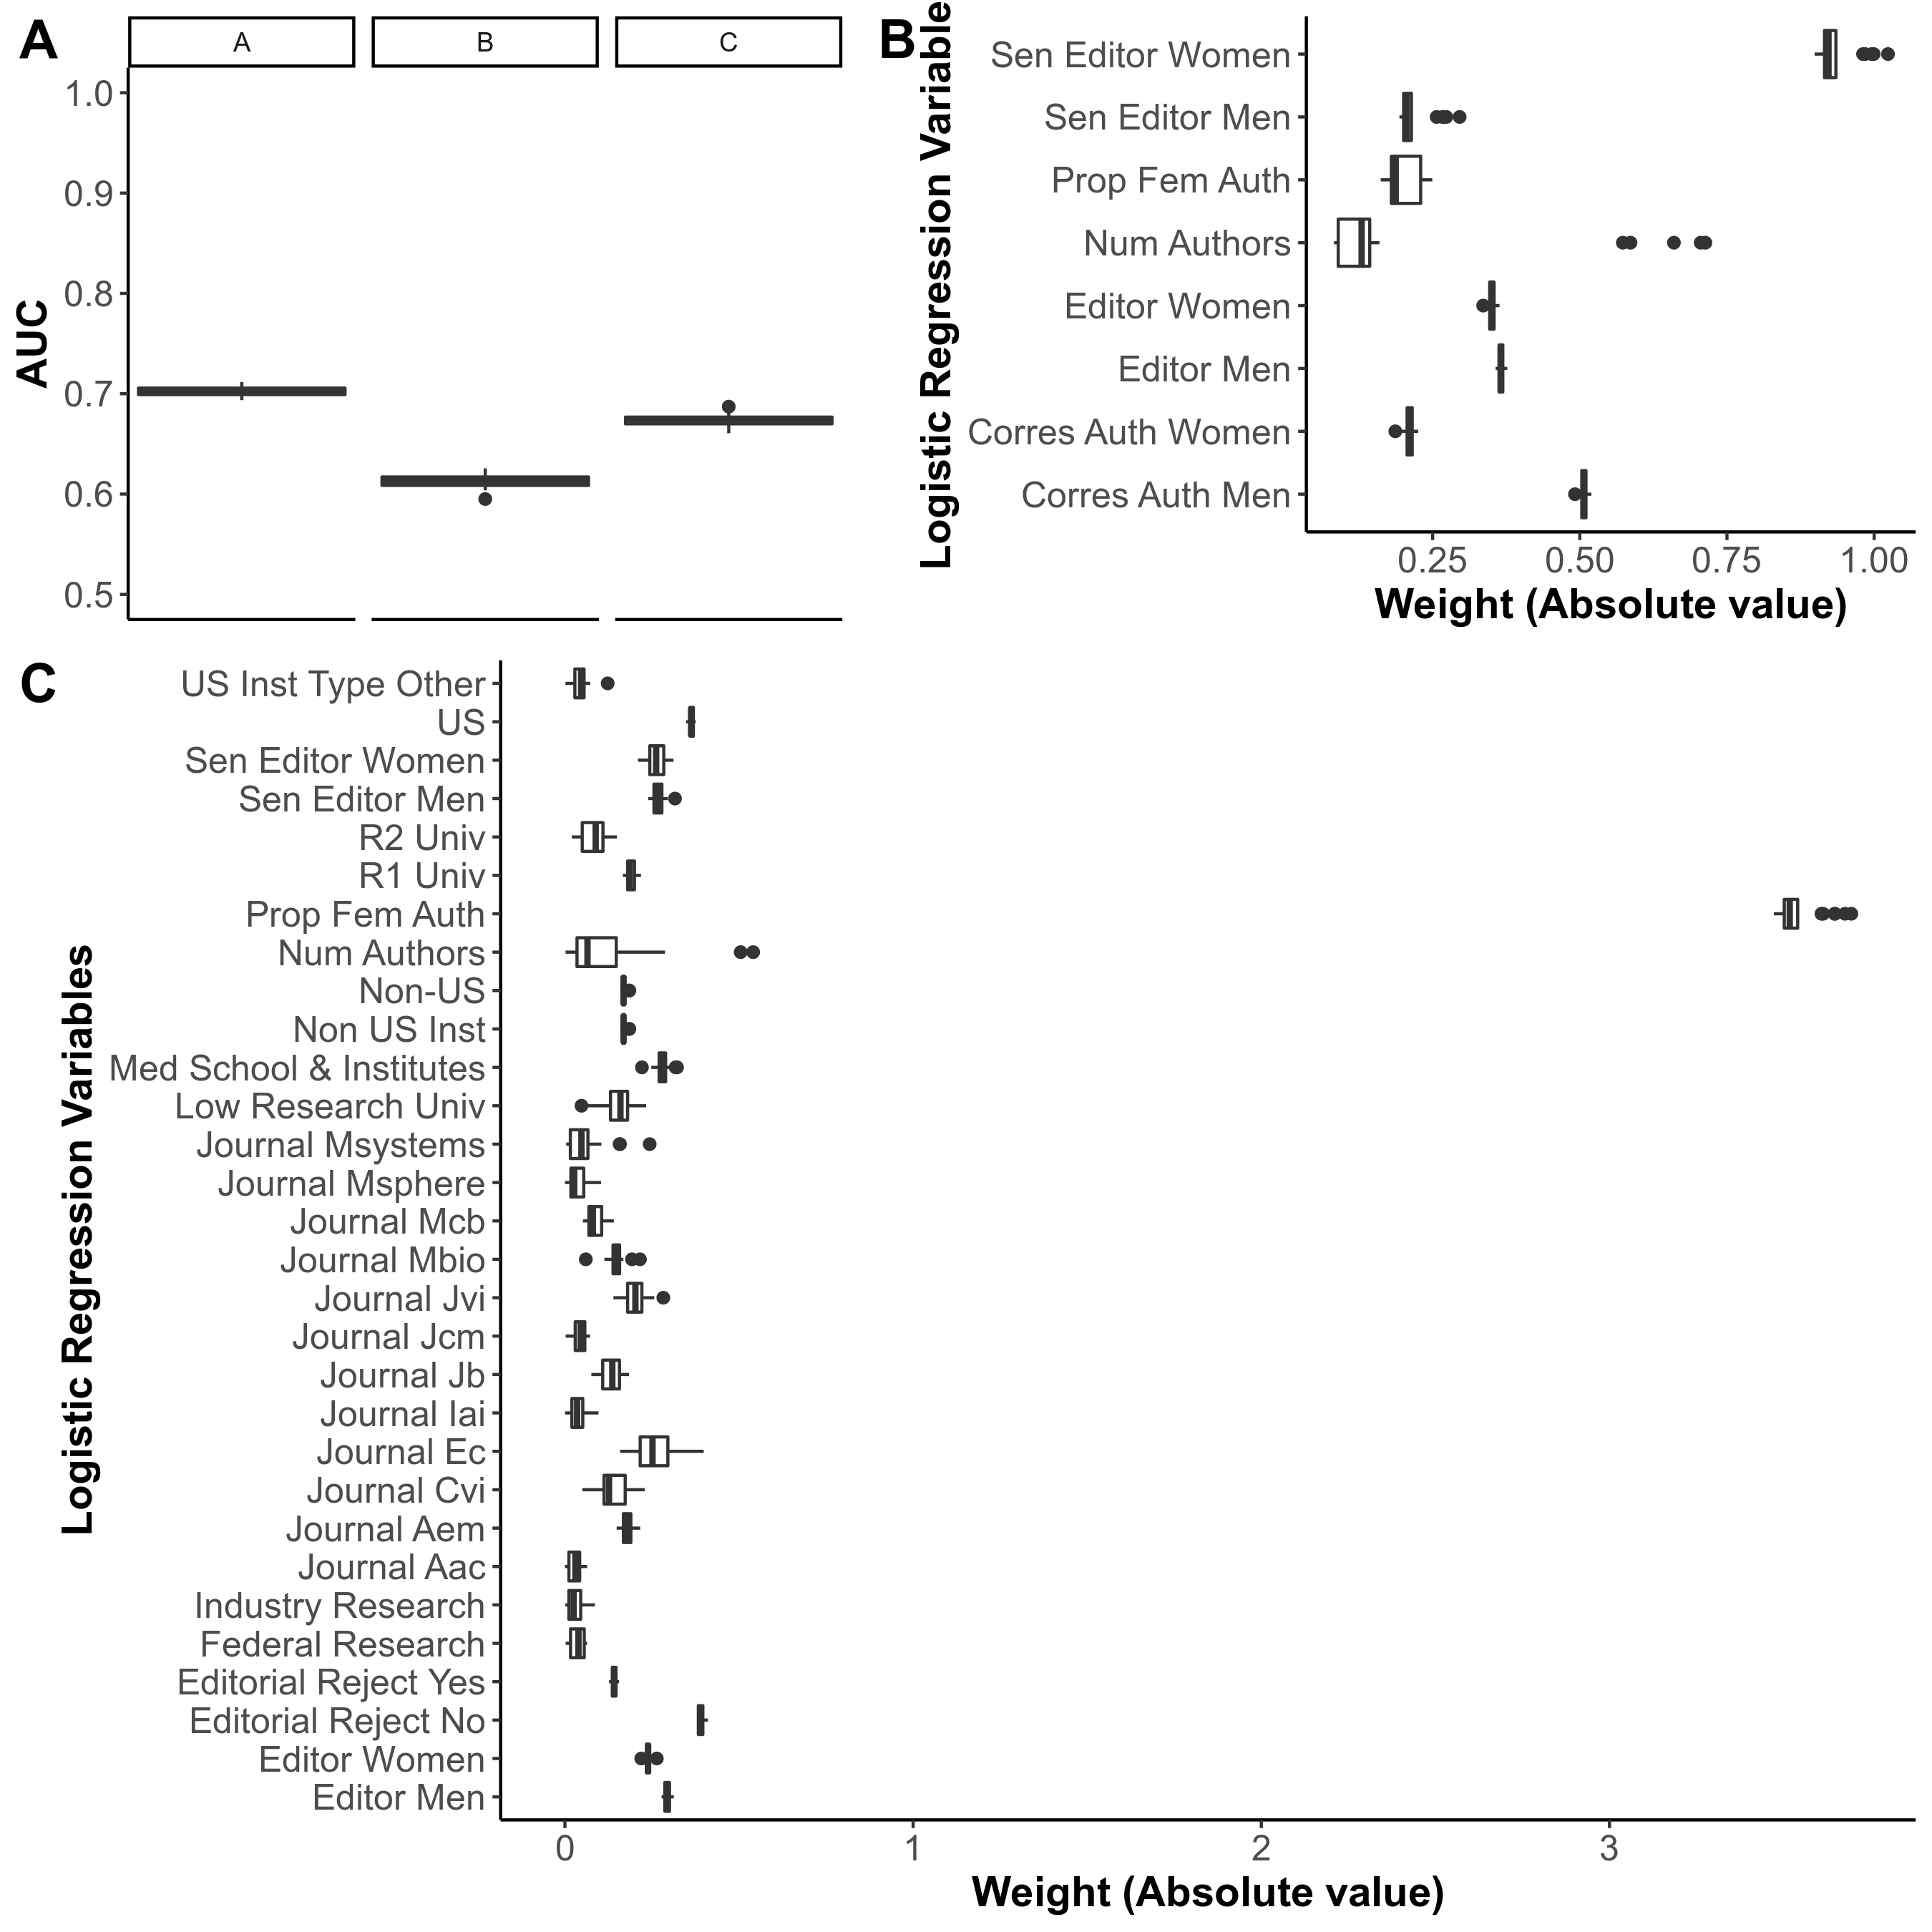
\includegraphics{Figure_S5.png} Figure S5. Comparison of time to final
decision and impact by gender. The number days (A) between when a
manuscript is initially submitted then finally published and (B) that a
manuscript spends in the ASM peer review system. How the impact of
papers published by men (blue) versus women (orange) vary according to
(C) cites and (D) total reads. Citation data includes articles published
between 36 and 48 months prior to August 2018. Total reads includes both
HTML and PDF online views for articles published between 12 and 24
months prior to August 2018. Impact data are divided by the number of
months published.

\newpage

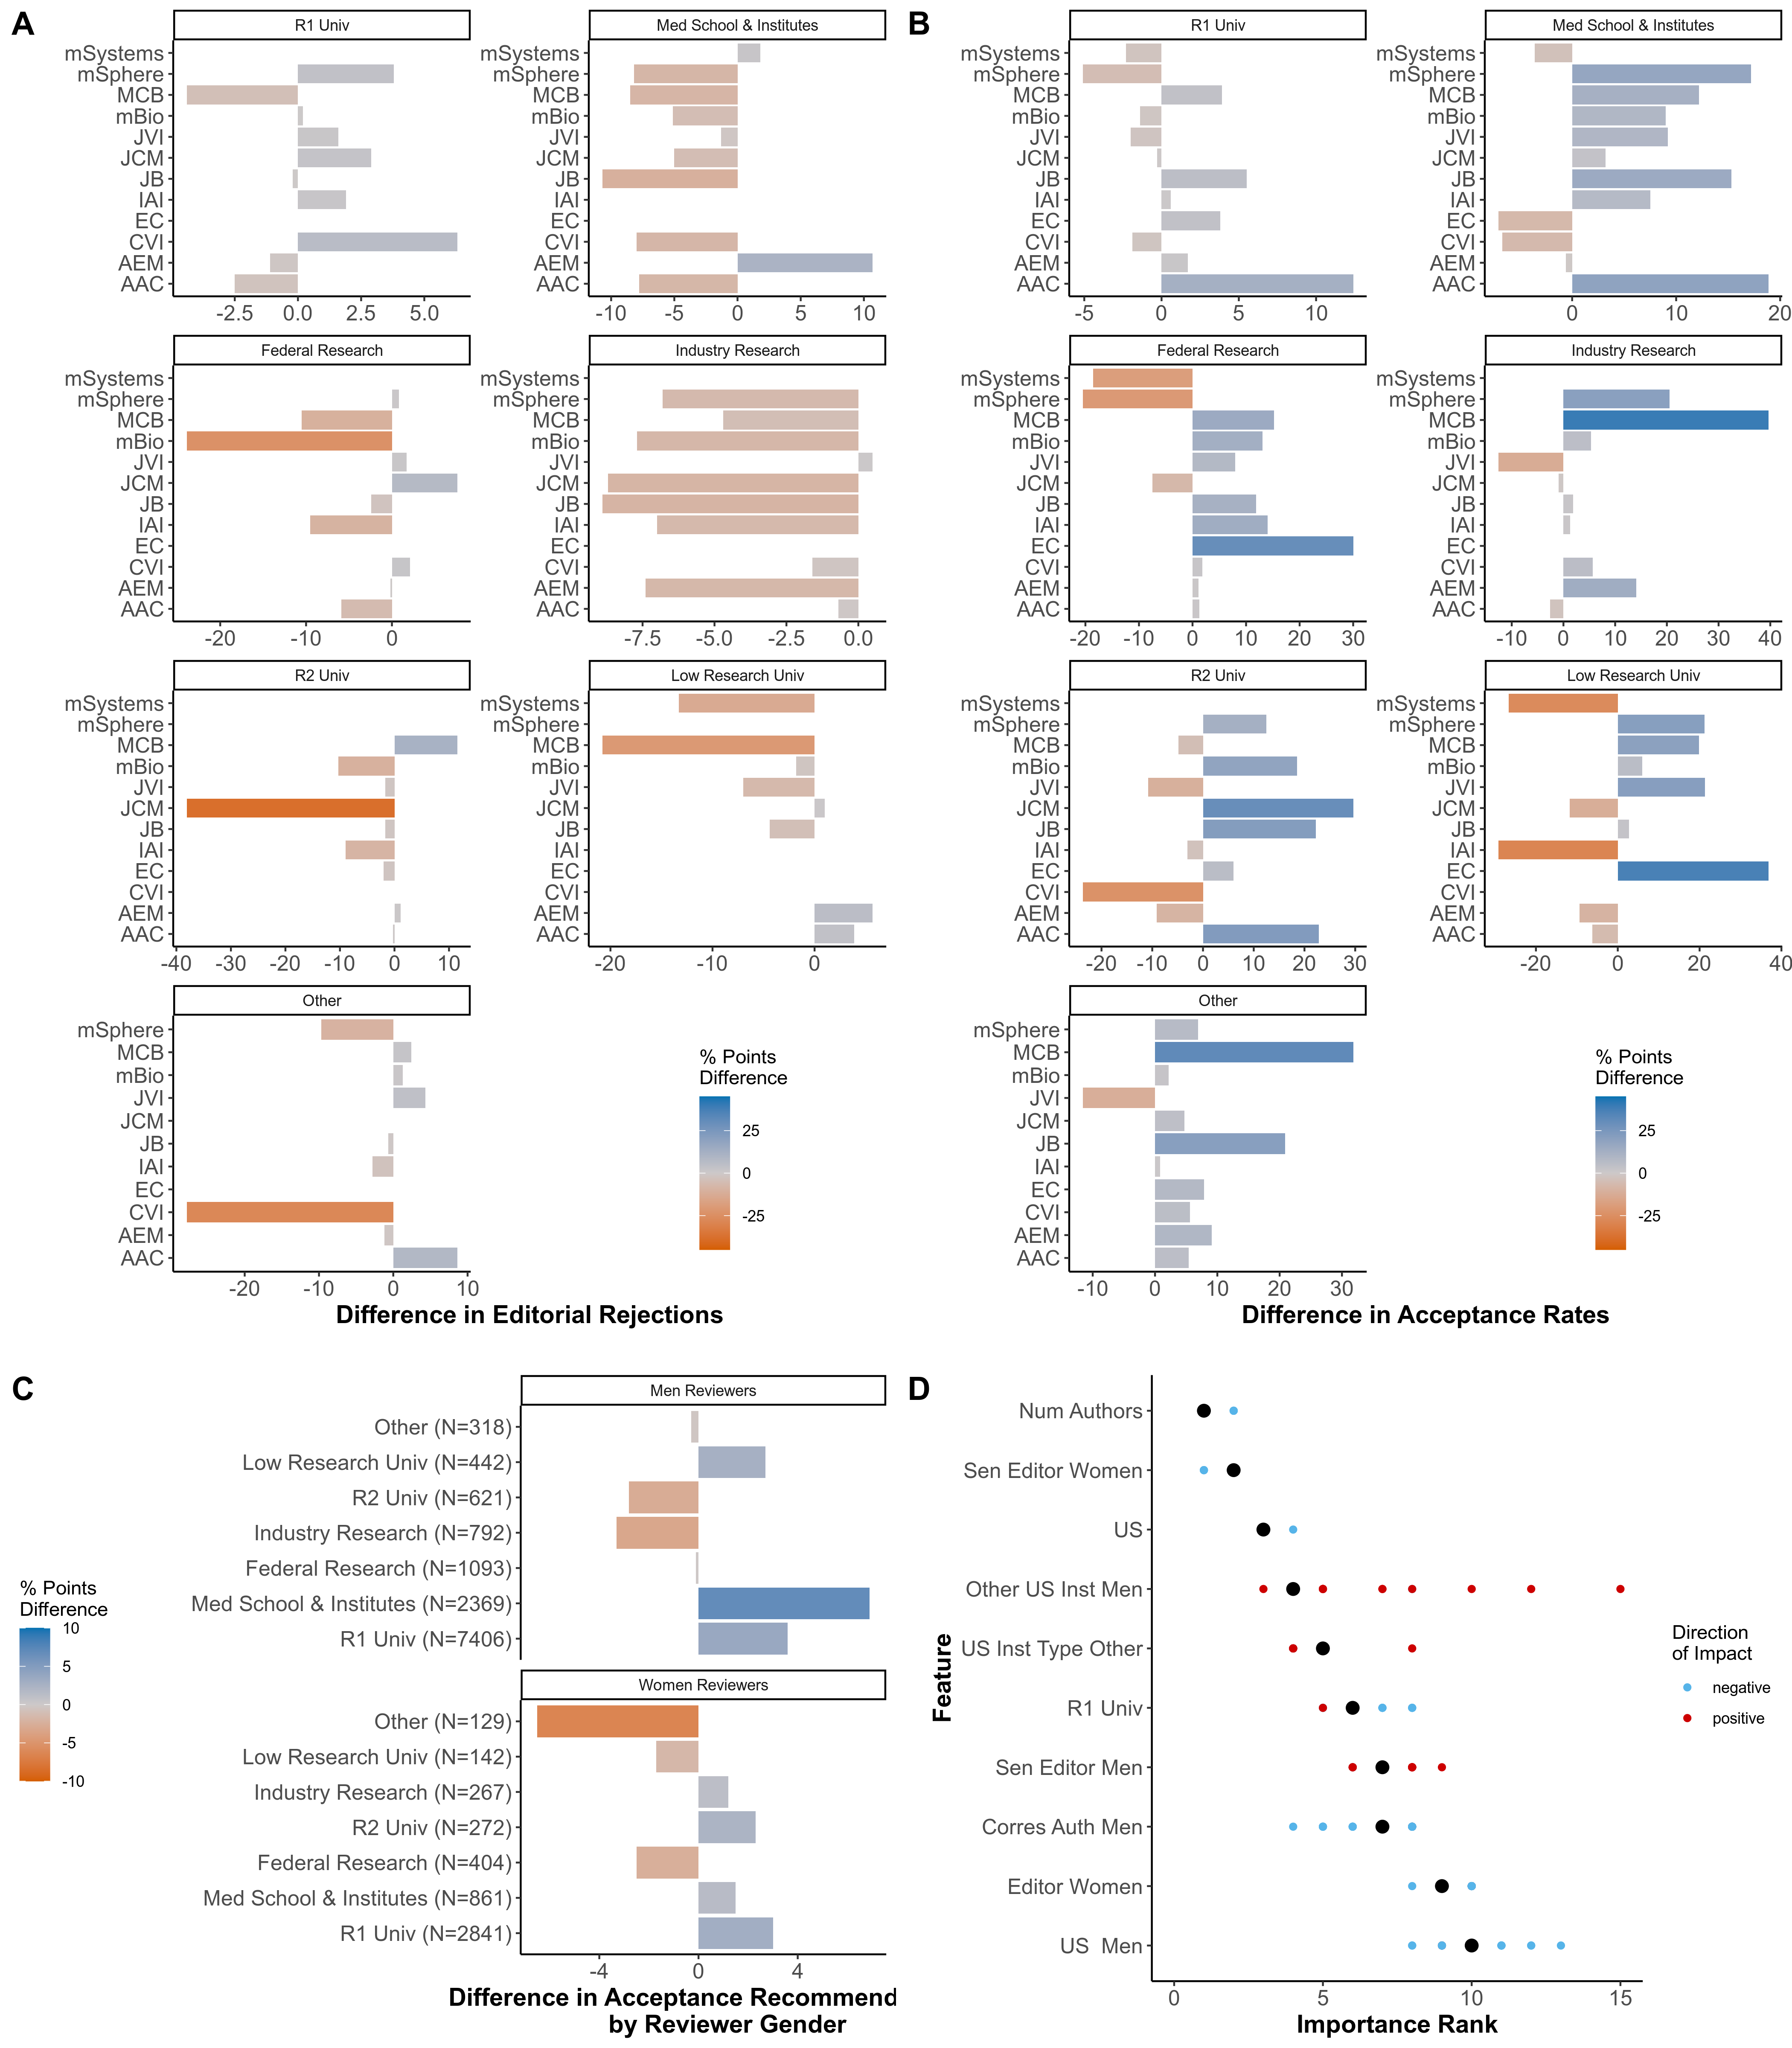
\includegraphics{Figure_S6.png} Figure S6. Difference in acceptance and
rejections by institution type.

\newpage

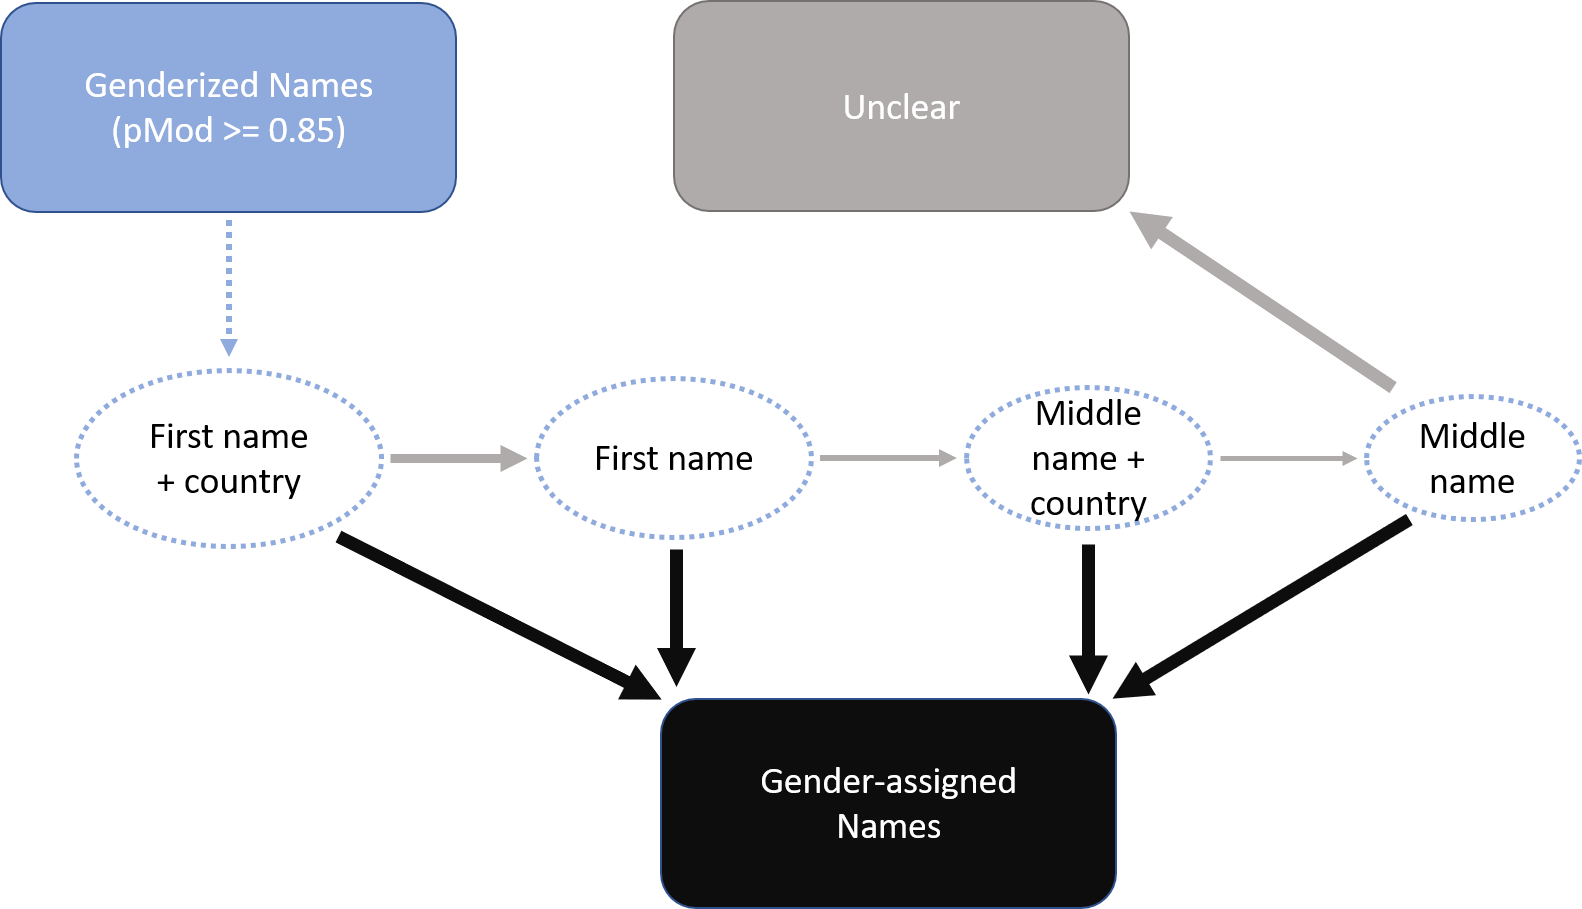
\includegraphics{genderize_method.png} Figure S7. Schematic of gender
prediction and assignment.

\newpage

Table S1. sensitivity/specificity/accuracy of genderize thresholds.
Bolded text denotes the accuracy of the threshold used in all further
analyses.

\begin{table}[H]
\centering
\begin{tabular}{l|r|r|l|r|r|l}
\hline
\multicolumn{1}{c|}{ } & \multicolumn{3}{c|}{First Names} & \multicolumn{3}{c}{Plus Country Data} \\
\cline{2-4} \cline{5-7}
Measure & p0.5 & p0.85 & pmod0.85 & p0.5 & p0.85 & pmod0.85\\
\hline
Sensitivity & 0.8943 & 0.9516 & \cellcolor{white}{0.971} & 0.9055 & 0.9471 & \cellcolor{white}{0.9669}\\
\hline
Specificity & 0.9339 & 0.9593 & \cellcolor{white}{0.972} & 0.9265 & 0.9553 & \cellcolor{white}{0.9727}\\
\hline
Accuracy & 0.9110 & 0.9549 & \textbf{0.9714} & 0.9146 & 0.9507 & \textbf{0.9695}\\
\hline
\end{tabular}
\end{table}

\vspace{40mm}


\includegraphics{impact_equation.png} Figure S8. Equation for
calculating negative bias by genderize. C indicates an individual
country.

\newpage

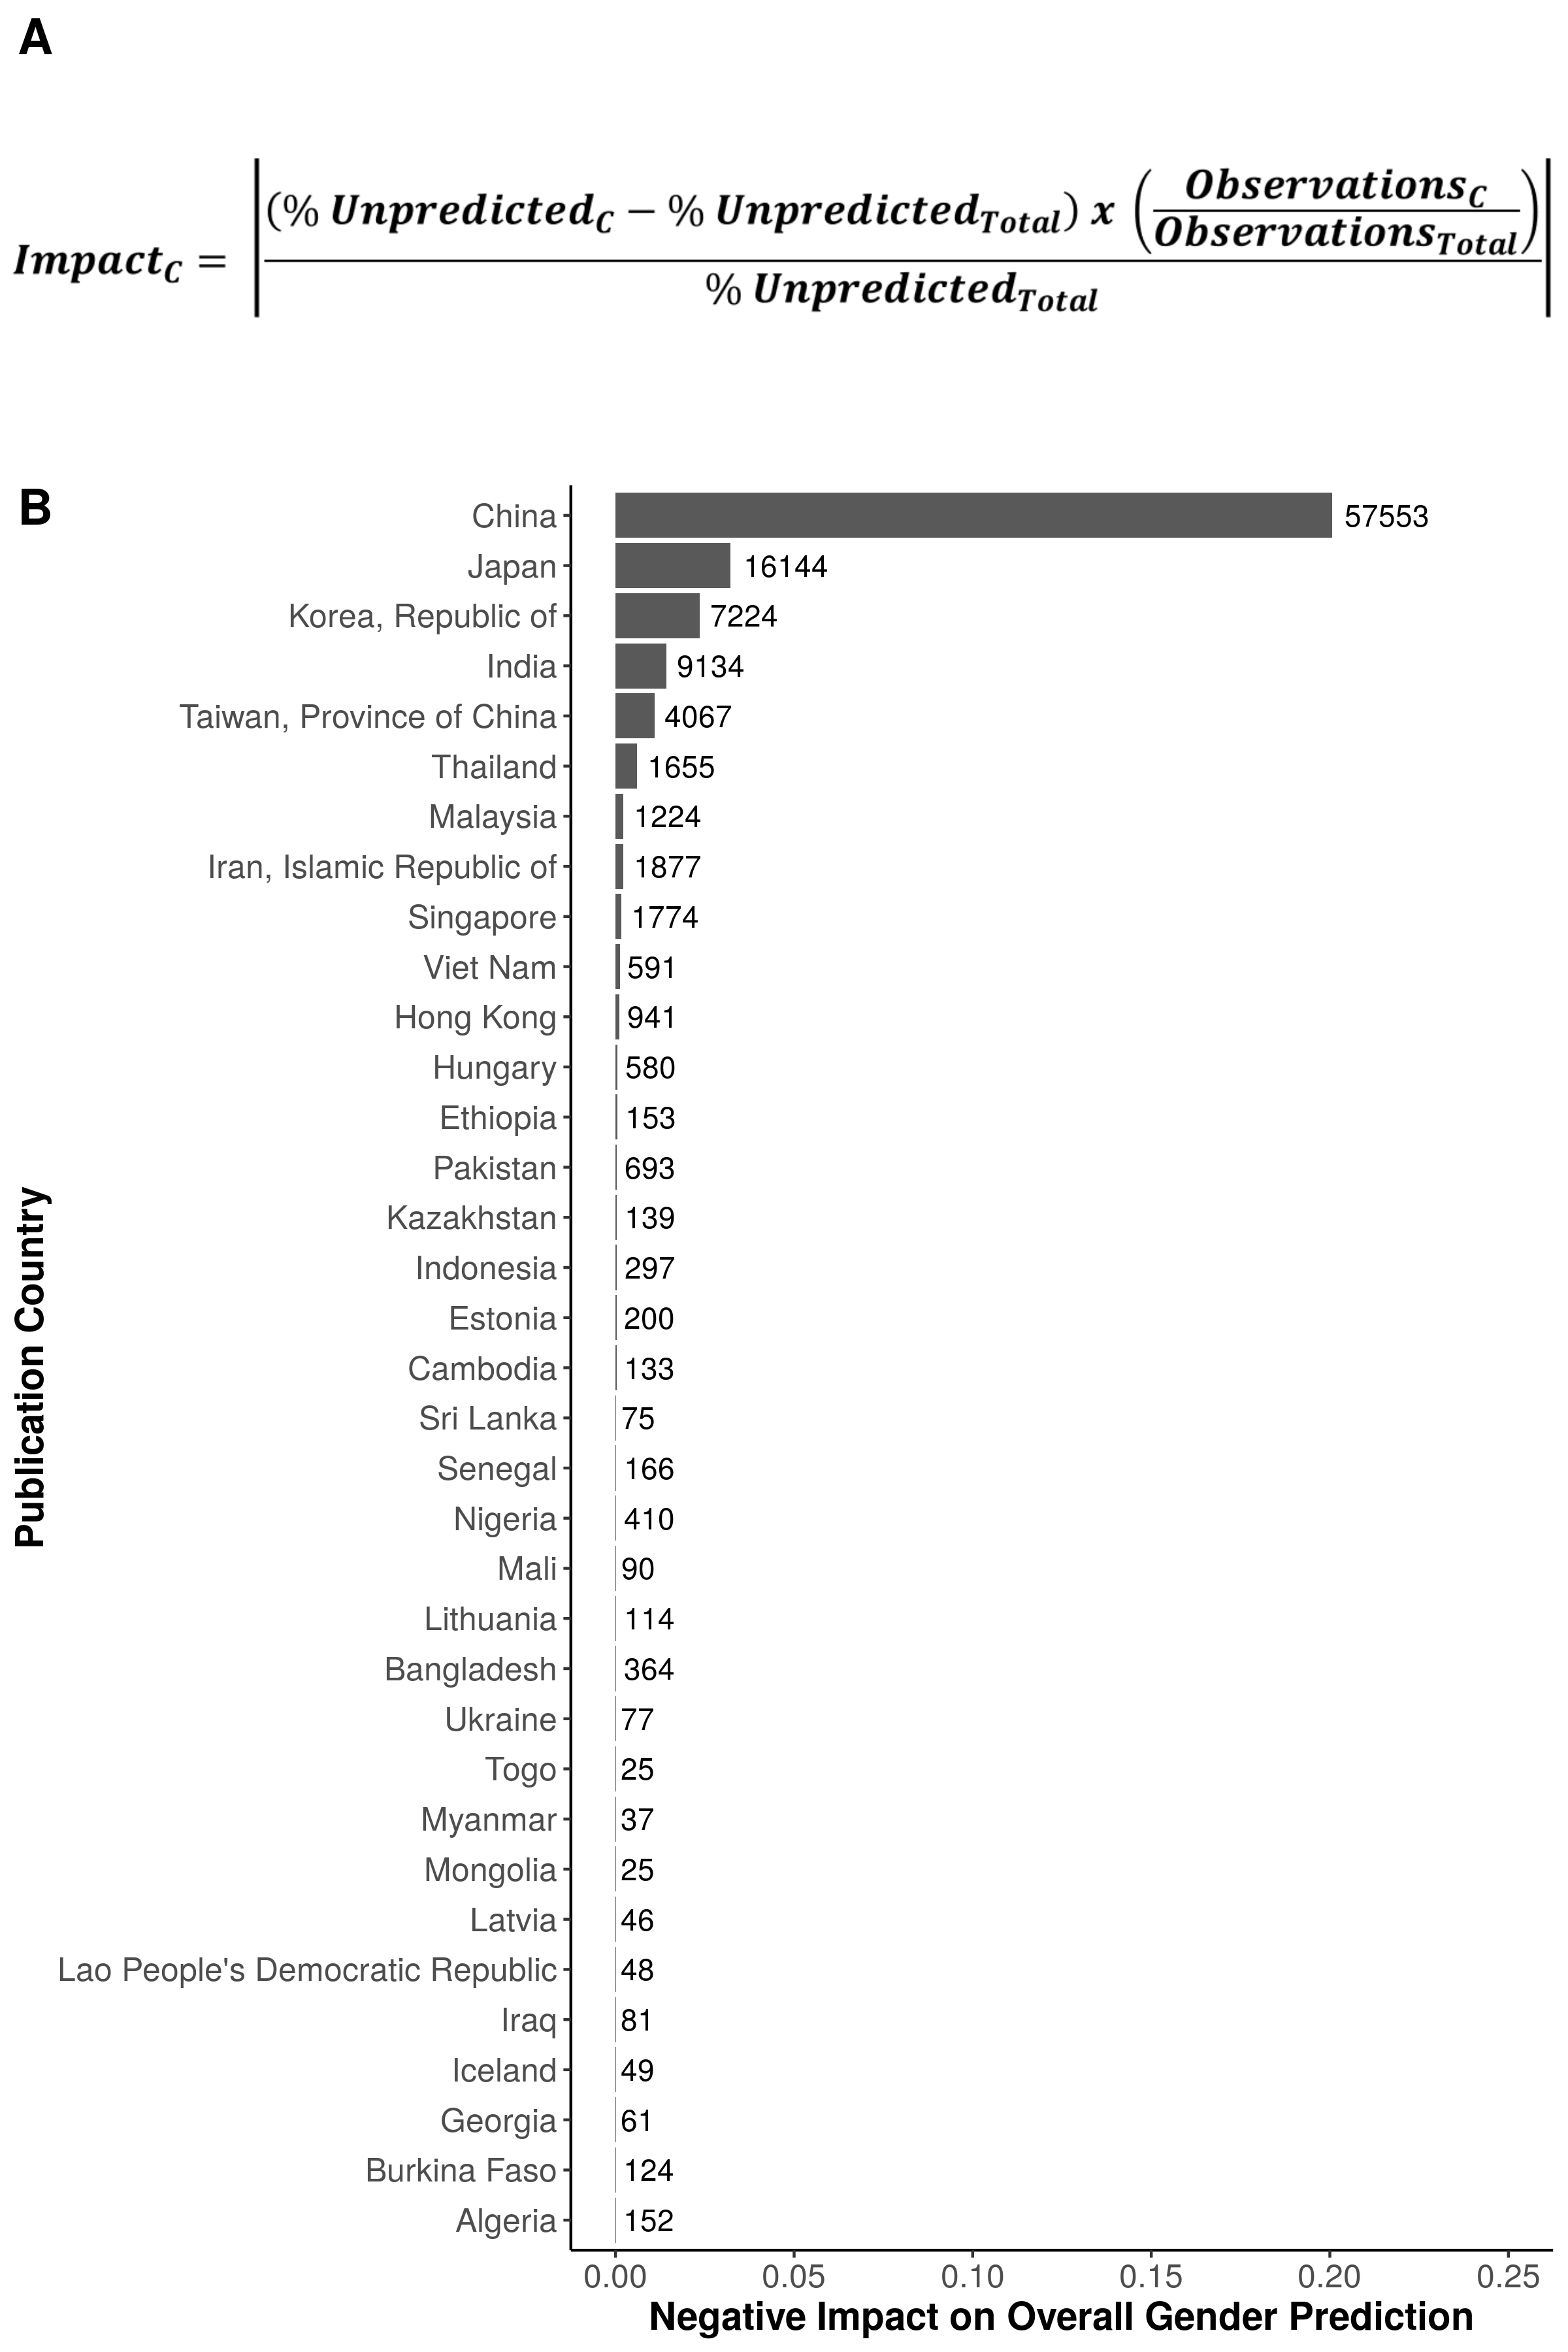
\includegraphics{Figure_S8.png} Figure S9. The negative impact of each
country on the overall gender prediction of the validation dataset.
Number indicates the total number of names associated with each country.

\newpage

\includegraphics{Figure_S9.png} Figure S10. The negative impact of each
country on the overall gender prediction of the full dataset. Number
indicates the total number of names associated with each country.

\subsection{References}\label{references}


\end{document}
